% TeX 
%
% Latex template for MIUN Licentiate/PhD thesis
% Author: David Krapohl
% Author: Winnie Wong
\input glyphtounicode                                               % use unicode for pdf
 \pdfgentounicode=1

% original 10pt
\documentclass[11pt,twoside,openright]{memoir}
%showtrims
\usepackage{fixltx2e}							%this package fixes some bugs in latex in case you have problems. I needed to use it in my thesis but don't remember for what

\usepackage[T1]{fontenc}
\usepackage[utf8]{inputenc}
\usepackage{textcomp}

\usepackage{etoolbox}

%\usepackage[ibycus,english,swedish,german]{babel}
\usepackage[english,swedish]{babel}

\usepackage{csquotes}
\usepackage{nicefrac}

% -- Graphics & Fonts & Colors
\usepackage{amssymb}
\usepackage{newpxtext,newpxmath}			% palatino (MIUN,serif)
%\usepackage{amsmath, pxfonts}				% palatino math
%\usepackage{gillius}						% gill sans (MIUN, sans)
\usepackage{helvet}							% helvetica as sans font

\usepackage{textgreek}

\usepackage[kerning=true,
            tracking=true,
            spacing=true,
            factor=1100,
            activate={true,nocompatibility},
            final]{microtype}				% even grayvalue, less rivers, optical edges
\SetTracking{encoding={*}, shape=sc}{40}	% nicer SC shape, less dense
\linespread{1.05}

\usepackage[toc,eqno]{tabfigures}	% set lining figures in tables

\usepackage[usenames,dvipsnames,cmyk]{xcolor}
    % define MIUN colors
    \definecolor{hiddenLink}{rgb}{0,0,0}
    \definecolor{miunBlue}{cmyk}{1,0.34,0,0.2}
    \definecolor{miunYellow}{cmyk}{0,0.1,1,0}
    \definecolor{miunBlack}{cmyk}{0,0,0,1}
    \definecolor{miunLightGray}{cmyk}{0,0,0,0.11}
    \definecolor{miunDarkGray}{cmyk}{0.11,0.11,0,0.69}

\usepackage[pdftex]{graphicx}
    \graphicspath{{./figures/}}

% useful extensions
\usepackage{makeidx}				

\usepackage{caption}                       % configure captions
%\usepackage{subcaption}
\usepackage{wrapfig}                        % wraps figure with text
\usepackage{float} 			% allows floating objects
%\usepackage[printonlyused]{acronym}        % print list of acronyms
\usepackage{booktabs}                       % beautify tables
\usepackage{multirow}                       % multiple rows in tables
\usepackage{siunitx}                        % make setting units fun and good looking 
\usepackage[version=3]{mhchem}              % nicer isotopes

\AtBeginEnvironment{tabularx}{%
    \figureversion{lf,tab}
    \sisetup{text-rm={\figureversion{tab,lf}}}
}
    \sisetup{detect-weight=true, detect-family=true, detect-mode=true, tight-spacing=true} % Make siunitx detect font-face and weight


%\usepackage[caption=false,font=footnotesize]{subfig}
\usepackage{subcaption}
    %\renewcommand{\arraystretch}{1}				  % more space in tables
%\usepackage{rotating}
\usepackage{longtable}
\usepackage{tabu}
\usepackage{gensymb}

\usepackage{enumitem}
% redefine the description environment
    \setlist[description]{%
        %    topsep=30pt,               	% space before start / after end of list
        %    itemsep=5pt,               	% space between items
        font={\normalfont\scshape}, % set the label font
        labelsep=\textwidth
    }

\usepackage{pdfpages}						% helps including pdf
\usepackage{tikz}							% graph drawing
\usepackage{pgfplots}						% plot in tikz
\pgfplotsset{compat=1.14}
% !Tex root = ../main.tex

\pgfplotsset{compat=1.10}
\usepgfplotslibrary{fillbetween}

\usetikzlibrary{arrows,positioning,snakes,shapes} 

% some tikz libraries
\usetikzlibrary{decorations.pathmorphing, decorations.pathreplacing, patterns}
\usetikzlibrary{circuits.ee.IEC}
\usetikzlibrary{calc}
% externalize all tikz figures: faster compilations
% pdf, log and md5sum is in tikz folder
\usetikzlibrary{external}
% externalize does not like includepdf
\tikzexternalize[prefix=tikz/, shell escape=-enable-write18, optimize command away=\includepdf]

\tikzset{
    %Define standard arrow tip
    >=stealth',
%    %Define style for boxes
%    point/.style={
%           rectangle,
%           rounded corners,
%           draw=black, very thick,
%           text width=6.5em,
%           minimum height=2em,
%           text centere},
	font=\sffamily,
    % Define arrow style
    arrow/.style={
           ->,
           thick,
           shorten <=2pt,
           shorten >=2pt,}
%    external/optimize=false
}
%some commands for figures that are reused
\newcommand{\electron}[1]{%
	\shade[ball color=darkgray] (#1) circle (.1);\draw (#1) node{};
}

\newcommand{\hole}[1]{%
	\shade[ball color=white] (#1) circle (.1);
}
%\tikzifexternalizing{% compile pgf only when it changes
%% don't include package XYZ here
%}{%
%\usepackage{pdfpages}% helps including pdf
%}%
\usepackage{hyperref}						% links in pdf document
\usepackage{tocloft}						%
\usepackage[noabbrev]{cleveref}				% clever refences (ranges,...)

% Color settings for the pdf file
    \hypersetup{
        hidelinks,
    %   backref=true,                       % bibliography links to text
    % 	bookmarks=true,
     	pdftitle={PDF title},
    	pdfauthor={Author},          %<<----TODO: author
    	colorlinks=false,                   % we use text colors
    %	linkcolor=hiddenLink,               % color for links...
    %	citecolor=hiddenLink,
    %	filecolor=link,
    %	menucolor=hiddenLink,
    %	urlcolor=hiddenLink,
    	bookmarksnumbered=true,             %
    	linkbordercolor=1. 1. 1.,           % frame around links->white
    	urlbordercolor = 1. 1. 1.           % frame around urls->white 
}

\usepackage[style=numeric,natbib=true,backend=bibtex8]{biblatex}
\addbibresource{./backmatter/licbib170609.bib}%{./backmatter/ref170411.bib}
%------------------------
%\usepackage[backend=biber,                  % configures bibliography, use biber
%            style=alphabetic,
%            maxcitenames=3,
%            maxbibnames=5,
%            firstinits=true,
%            url=false,
%            isbn=false,
%            autolang=other
%            ]{biblatex}
%%-------------------------
%%    \appto{\bibsetup}{\raggedright}        
%    \DeclareSourcemap{% used for mapping language to hyphnation in bibtex 
%        \maps{
%            \map{
%                \step[fieldsource=language, fieldset=langid, origfieldval, final]
%                \step[fieldset=language, null]
%            }
%        }
%    }
%}            


%\bibliography{./backmatter/reflib170328} 

\usepackage[nomain,%
            nopostdot,%
            acronym,%
            toc,%
            nonumberlist,
            translate=babel]{glossaries}		% glossary package for acronyms
\makeglossaries


%%% TEST/DRAFT packages, disable in final! ===================

%\usepackage[l2tabu, orthodox]{nag}	% added 21/01/14 by DK
\usepackage[colorinlistoftodos]{todonotes}
\usepackage{blindtext}
%\usepackage{layouts}
%%% Other Useful Packages (Added 02/05/12 by WW)

%\usepackage{lineno} %add line numbers to draft copies
%\linenumbers
%\setpagewiselinenumbers

%%% END TEST/DRAFT packages ==================================

%\usepackage{mdwlist} % remove white space between lists


% -- Layout ------------------------------------------------
% .. page size .............................................
\setstocksize{240mm}{169mm} % this is the real size
\settrimmedsize{\stockheight}{\stockwidth}{*}

% trimmarks (use for measuring when printing A4 paper)
%\setstocksize{297mm}{210mm}
%\trimFrame
%\settrimmedsize{240mm}{170mm}{*}
%\settrims{2cm}{2cm}

\setbinding{5mm}
\settypeblocksize{*}{115mm}{1.6} % davkra 2015-02-24
% spine, edge, ratio
\setlrmargins{20mm}{*}{*}
% upper lower, ratio
\setulmargins{*}{*}{1.2}


% .. page layout ...........................................
% .. headers and footers
\makepagestyle{miunlic}
\makeevenhead{miunlic}{\small\leftmark}{}{}
\makeoddhead{miunlic}{}{}{\small\rightmark}
\makeevenfoot{miunlic}{\small page | \thepage}{}{}
\makeoddfoot{miunlic}{}{}{\small page | \thepage}

\makeatletter % because of \@chapapp
\makepsmarks {miunlic}{%
  \nouppercaseheads
  \createmark{chapter}{both}{shownumber}{\@chapapp\ }{. \ }
  \createmark{section}{right}{shownumber}{}{. \ }
  \createmark{subsection}{right}{shownumber}{}{. \ }
   %TODO: decide subsub or subsection
  \createplainmark {toc}{both} {\contentsname}
  \createplainmark {lof}{both} {\listfigurename}
  \createplainmark {lot}{both} {\listtablename}
  \createplainmark {bib}{both} {\bibname}
  \createplainmark {index}{both} {\indexname}
  %\createplainmark {glossary}{both} {\glossaryname}
}
\makeatother

% .. adjust plain style too
\makeevenfoot{plain}{\small page | \thepage}{}{}
\makeoddfoot {plain}{}{}{\small page | \thepage}

% .. table of contents .....................................
\renewcommand{\cftchapterfont}{\scshape}
\renewcommand{\cftchapterpagefont}{\scshape}
%\renewcommand{\cftsectiondotsep}{\cftnodots}

% .. numbering depth
\setsecnumdepth{subsection}
\maxsecnumdepth{subsection}

% .. numbering depth
\maxtocdepth{section}
\settocdepth{section}
% .. text separators........................................
% .. parts
%\renewcommand{\partnamefont}{\LARGE}
%\renewcommand{\partnumfont}{\scshape\LARGE}
%\renewcommand{\parttitlefont}{\color{miunBlue}\scshape\huge}
%\renewcommand{\cftpartfont}{\color{miunBlue}\scshape}
%\renewcommand{\parttitlefont}{\scshape\huge} % minimize color usage 21/01/14 by DK
%\renewcommand{\cftpartfont}{\scshape}
%
%\renewcommand{\cftpartpagefont}{\scshape}

% .. chapter style
\headstyles{bringhurst}
%\chapterstyle{pedersen}
%\chapterstyle{chappell}


% these commands go into chapter titles
\def\Vhrulefill{\leavevmode\leaders\hrule height 0.7ex depth \dimexpr0.4pt-0.7ex\hfill\kern0pt}

\def\nbrcircles{100}%100! 247 377
\def\outerradius{10mm} 
\def\deviation {.9}
%\def\fudge {.62}
\def\fudge {.27}

% the chapter style
\makeatletter 
\makechapterstyle{dots}{%
    \chapterstyle{default}
    \renewcommand*{\chapterheadstart}{}
    \renewcommand*{\printchaptername}{%
        \centerline{\parbox{0.5cm}{\Vhrulefill} \chapnumfont{\@chapapp\ \thechapter} \parbox{0.5cm}{\Vhrulefill}}}
    \renewcommand*{\chapternamenum}{}
    % \renewcommand*{\chapnumfont}{\normalfont\scshape\MakeTextLowercase}
    \renewcommand*{\chapnumfont}{\normalfont\sffamily}
    \renewcommand*{\printchapternum}{}
    \renewcommand*{\afterchapternum}{\vspace{2mm}
        %
        %\par\centerline{\parbox{0.5in}{\hrulefill}}\par
    }
    \renewcommand*{\afterchaptertitle}{\par\nobreak\vskip0.5\midchapskip}
    \renewcommand*{\printchapternonum}{%
        \vphantom{\chapnumfont \@chapapp 1}\par
        \parbox{0.5in}{}\par}
    \renewcommand*{\chaptitlefont}{\normalfont\sffamily\Huge}
    \renewcommand*{\printchaptertitle}[1]{%
        \centering \chaptitlefont\MakeTextUppercase{##1}\\
    }}
\makeatother
\chapterstyle{dots}

% .. sections
%\setsecheadstyle{\scshape\large}
\setsecheadstyle{\large\sffamily}
\setsubsecheadstyle{\itshape\sffamily}
\setsubsubsecheadstyle{\itshape\sffamily\small}
% .. captions
\captionnamefont{\sffamily\footnotesize}
\captiontitlefont{\sffamily\footnotesize}

%\subcaptionlabelfont{\sffamily\footnotesizefd}
%\subcaptionfont{\sffamily\footnotesize}
%\changecaptionwidth
%\captionwidth{0.75\textwidth}

\captionsetup[subfigure]{font={scriptsize,sf}}
\captionsetup[figure]{width=\textwidth}

\setfloatadjustment{figure}{\centering}
% finalize it!
\checkandfixthelayout

% !TeX root = main.tex
% !TeX spellcheck = en_GB


\hyphenation{Me-trop-olis}


%\newcommand{\galpha}{\ibygr{a}}
%\newcommand{\gbeta}{\ibygr{b}}
%\newcommand{\ggamma}{\ibygr{g}}
%\newcommand{\gdelta}{\ibygr{d}}
%\newcommand{\gDelta}{\ibygr{D}}
%\newcommand{\gepsilon}{\ibygr{e}}

\newcommand{\galpha}{\textalpha}
\newcommand{\gbeta}{\textbeta}
\newcommand{\ggamma}{\textgamma}
\newcommand{\gdelta}{\textdelta}
\newcommand{\gDelta}{\textDelta}
\newcommand{\gepsilon}{\textepsilon}

\newcommand{\mff}{\SI{55}{\micro\meter}}
\newcommand{\mht}{\SI{110}{\micro\meter}}
\newcommand{\threeh}{\SI{300}{\micro\meter}}
%\newcommand{\FIXME}{\noindent\hrulefill FIXME \hrulefill}
\newcommand*\FIXMEl{\color{red}\par\noindent\raisebox{.8ex}{\makebox[\linewidth]{\hrulefill\hspace{1ex}\raisebox{-.8ex}{FIXME}\hspace{1ex}\hrulefill}}\color{black}}
\newcommand{\FIXME}{\color{red}FIXME\ \color{black}}
% faster medipix commands
\newcommand{\mpx}[1][]{\textsc{Medipix#1}}
\newcommand{\tpx}[1][]{\textsc{Timepix#1}}
% neutron detector
%\newcommand{\tib}{\ce{TiB2}}
\newcommand{\tib}{\ce{TiB2}}
% Define the command. Note that the input and output folders are static!
%\newcommand{\includetikz}[1]{%
%	\input{figures/#1.pgf}%
%}

% inputtikz command for figures
\newcommand*{\inputtikz}[2]{%
\resizebox*{#1\textwidth}{!}{%
\input{figures/#2}}}

% we need this for correct label references to papers
\newcounter{dummy}

% -- empty page commands --
%\newcommand\emptypage{\newpage\null\thispagestyle{empty}\newpage}   % inserts empty page (empty)
%\newcommand\emptypagenum{\newpage\null\thispagestyle{plain}\newpage}% inserts empty page (plain)

% commands only for editing:
% do not externalize the \todo command
\makeatletter
\renewcommand{\todo}[2][]{\tikzexternaldisable\@todo[#1]{#2}\tikzexternalenable}
\makeatother



\newcommand{\todocite}[1]{\todo[color=yellow, author=cite]{#1}}


%\glsdefmain{main}
%\makeglossaries
%\input{./backmatter/glossary} %folder added by WW 02/05/12
%% !TeX root = ../main.tex
\newacronym{lwc}{LWC}{Liquid Water Content}
\newacronym{mvd}{MVD}{Median Volume Diameter}
\newacronym{led}{LED}{light emitting diode}
\newacronym{cmos}{CMOS}{Complementary Metal Oxide Semiconductor}
\newacronym{log}{LoG}{Laplacian of Gaussian}
\newacronym{dii}{DII}{Droplet Imaging Instrument}
\newacronym{cdp}{CDP}{Cloud Droplet Probe}
\newacronym{smhi}{SMHI}{Sveriges meteorologiska och hydrologiska institut, (Swedish Meteorological and Hydrological Institute)}
\newacronym{arome}{AROME}{Application de la Recherche à l'Opérationnel à Méso Echelle, (Application of Research to Operations at Mesoscale)}
\newacronym{nwp}{NWP}{Numerical Weather Prediction}
\newacronym{lam}{LAM}{Limited Area Models}
\newacronym{snr}{SNR}{signal to noise ratio}
\newacronym{oap}{OAP}{Optical Array Probe}
\newacronym{nist}{NIST}{National Institute of Standards and Technology}
\newacronym{dmt}{DMT}{Droplet Measurement Technologies}
\newacronym{twc}{TWC}{True Water Content}
\newacronym{ecmwf}{ECMWF}{European Centre for Medium-Range Weather Forecasts}
\newacronym{harmonie}{HARMONIE}{HIRLAM (High Resolution Local Area Modelling)–ALADIN (Aire Limitée Adaptation dynamique Développement InterNational) Research on Mesoscale Operational NWP (Numerical Weather Prediction) in Europe} %folder added by WW 02/05/12


%
% \\\\\\\\\\\\\\\\\\\\\\ THE THESIS ////////////////////////
%

% !TeX root = main.tex
% !TeX spellcheck = en_GB
%: title
%TODO:
\title{Measuring Water Droplets to Detect Atmospheric Icing}
\author{Staffan Rydblom}
\date{\today}

\newcommand{\theSupervisor}{Associate Professor Benny Thörnberg,\\ Professor Mattias O'Nils}
\newcommand{\theThesisNumber}{XX}
\newcommand{\theISSN}{XXXX-XXXX}
\newcommand{\theISBN}{XXXX-XXXX} %added by WW 02/05/12 note: you can request these numbers from the library at http://www.bib.miun.se/eng/researchers/publishing/theses/preparations
%\newcommand{\subtitle}{Monte Carlo and Charge transport simulation in Medipix detector systems}


%-----------------------------------------------------------
% DON’T TOUCH THIS!
%\newlength{\drop}
\newcommand*{\titleCC}{\begingroup%
%\drop=0.0\textheight
%\vspace*{\drop}
\centering 
{Thesis for the degree of Licentiate of Technology\\
Sundsvall 2017}\\[1.5cm]
\par
{\huge \thetitle}\\[0.25cm]
{\Large\subtitle}\\[1.25cm]

\par
{\Large \theauthor}\\[.75cm]
\par
{Supervisor: \theSupervisor}\\[.75cm]
\par
{Department of Electronics Design, in the\\
Faculty of Science, Technology and Media\\
Mid Sweden University, SE-851 70 Sundsvall, Sweden}\\[0.75cm]
\par
{ISSN \theISSN}\\[0.75cm]
{ISBN \theISBN}\\[0.75cm] % added by WW 02/05/12
\par
{Mid Sweden University Licentiate Thesis \theThesisNumber}\\[0.75cm]
\vfill
%{\includegraphics[width=0.4\textwidth]{./figures/ElectronicsDesign_logo}}\\[0.2cm] % added by WW 02/05/12 note: if you use this logo, you might want to reduce the MIUN logo to width=0.4\textwidth
{
\includegraphics[width=0.5\textwidth]{./figures/MIUN_logotyp}}\\[0.5\baselineskip] %folder added by WW 02/05/12
%\vfill
\clearpage
\endgroup}


\pagestyle{miunlic}

\begin{document}

\renewcommand{\arraystretch}{1.2}
% -- frontmatter -------------------------------------------

\frontmatter
% .. titles ................................................
%todo remov in final
%\listoftodos
\newpage
\thispagestyle{empty}
\titleCC
% !Tex root = ../main.tex
\thispagestyle{empty}

{\raggedright
Akademisk avhandling som med tillstånd av Mittuniversitetet i Sundsvall framläggs till offentlig för avläggande av licentiatexamen i elektronik \textbf{onsdagen den 1 november 2017}, klockan \textbf{10.00} i sal \textbf{O102}, Mittuniversitetet Sundsvall. Seminariet kommer att hållas på engelska.

\vfill

{\large\thetitle}

\vspace{1cm}

\theauthor

\vspace{1cm}

\textcopyright  \theauthor, 2017
\vspace{1cm}

Faculty of Science, Technology and Media,
Mid Sweden University, SE-851 70 Sundsvall
Sweden

\vspace{1cm}

Telephone: +46 (0)60 148422

\vspace{1cm}

Printed by Mid Sweden University, Sundsvall, Sweden, 2017
} %folder added by WW 02/05/12
% .. dedication ............................................
\cleardoublepage
\null\vspace{\stretch{2}}
\begin{flushright}
	% !TeX root = ../main.tex
% !TeX spellcheck = en_GB
%: dedication

\vspace{4cm}
This is dedicated to...
 %folder added by WW 02/05/12
\end{flushright}
\vspace{\stretch{1}}\null

% .. start english abstract ................................
\selectlanguage{english}
\abstractintoc
\abstractnum

% !TeX root = ../main.tex
% !TeX spellcheck = en_GB
%: Abstract english
\begin{abstract}

This thesis describes the exploration of a method to measure the droplet size and the concentration of atmospheric liquid water. The purpose is to find a cost efficient technique to detect the conditions for icing on structures.

Icing caused by freezing atmospheric water can be a significant problem for infrastructure such as power lines, roads and air traffic. About one third of the global installed wind power capacity is located in cold climates, where icing of rotor blades is one of the major challenges. 

The icing process is complex and the result depends on a combination of the aerodynamic shape of the structure or airfoil, the velocity of the air and its contained water, the temperature, the mixing of snow and water, the concentration of liquid water and the droplet size distribution.

The chosen measurement method is based on a shadowgraph imaging system using \gls{led} light as background illumination and digital image processing. A prototype instrument has been constructed. The components were selected keeping the possibility of low-cost volume production in mind. The applications of a commercial instrument based on this technique are e.g. real-time in-situ icing condition measurements and assimilation and verification of data in numerical weather models.

The work presented shows that measurements of the size and concentration of water droplets using shadowgraph images can be used for the comparison and validation of \gls{nwp} models and other instruments. The accuracy of the particle size measurement is high. The accuracy of the concentration measurement has the potential to become high due to the single-particle measurement range calibration. The precision of the instrument depends mainly on the number of images that is used to find each measurement value. The real-time performance of the instrument is limited by the image retrieval and processing speed and depends on the precision required.

\end{abstract} %folder added by WW 02/05/12
\clearpage

% .. start swedish abstract ................................
\selectlanguage{swedish}
\abstractintoc

% !TeX root = ../main.tex
% !TeX spellcheck = en_SV
%: Abstract swedish


\begin{abstract}
Den här avhandlingen handlar om...
\end{abstract} %folder added by WW 02/05/12
\clearpage

% .. start toc,lof,lot .....................................
\selectlanguage{english}
\tableofcontents
\clearpage
\listoffigures
\clearpage
\listoftables
\clearpage %line added by WW 02/05/12
% !TeX root = ../main.tex

%\chapter{List of Papers}

\thispagestyle{plain}

\chapter*{List of Papers}
%\noindent {\Huge\bfseries\sffamily List of Papers}\\
\refstepcounter{dummy}
\addcontentsline{toc}{chapter}{List of Papers}
\vspace{20pt}

\noindent This thesis is based on the following papers, herein referred to by their Roman numerals:  

% paper name in a short command
\newcommand{\paperone}{Liquid Water Content and Droplet Sizing Shadowgraph Measuring System for Wind Turbine Icing Detection}
\newcommand{\papertwo}{Droplet Imaging Instrument - Metrology Instrument for Icing Condition Detection}
\newcommand{\paperthree}{Comparative Field Study of LWC and MVD using two Droplet Measuring Instruments and a NWP Model}

% authors in a short command
\newcommand{\authorone}{S.Rydblom, B. Thörnberg}
\newcommand{\authortwo}{S.Rydblom, B. Thörnberg, E. Olsson}


%some journals in short
\newcommand{\ieeesens}{IEEE Sensors Journal}
\newcommand{\ieeeconf}{IEEE International Conference on Imaging Systems and Techniques (IST) Proceedings}
\newcommand{\mst}{Measurement Science and Technology}
\newcommand{\coldreg}{Under Review for Cold Regions Science and Technology}

\begin{description}[style=nextline]
    \item[Paper I]
    \paperone \\ 
    \authorone, \ieeesens, 2015\dotfill \pageref{pap:paper1}
    
    \item[Paper II]
    \papertwo \\ 
    \authorone, \ieeeconf, 2016\dotfill \pageref{pap:paper2}
     
    \item[Paper III]
    \paperthree \\ 
    \authortwo, \coldreg, 2017\dotfill \pageref{pap:paper3}

%    \item[Paper V]
%    
%    \item[Paper VI]
%   
%    \item[Paper VII]
%
%    \item[Paper VIII]



\end{description}

 %line added by WW 02/05/12
\microtypesetup{protrusion=true}
%\printglossary[style=long4colheader, title=Glossary]


% .. start acknowledgment ..................................
% !TeX root = ../main.tex
% !TeX spellcheck = en_Gb

\chapter{Acknowledgements}

I would like to express the greatest gratitude to my supervisor, Benny Thörnberg, for his trust and encouragement especially when things did not turn out the way they were expected.
I would also like to thank Mattias O'Nils and Claes Mattsson at the Department of Electronics Design for making the project possible and giving me the possibility to finish the thesis.

I owe a big thanks to the Swedish Energy Agency for funding most of the work; Patrik Jonsson, Björn Ollars and Olof Carlsson at Combitech for their work with integration of the rotating mast and the CDP; and Esbjörn Olsson at SMHI for sharing his knowledge about the weather physics and his work with the NWP model data.

To my wonderful family; the greatest love and gratitute that have sacrificed a lot and supported me in beginning, fulfilling and finishing this work. Without you this would not have been possible.

Special thanks to Lotta Frisk, Fanny Burman, Carolina Blomberg, Christine Grafström and Maria Rumm for all the administrative work, inspiration and positive energy at the Department of Electronics Design.

Not forgetting my mentor Magnus Engholm, Vincent Skerved, Göran Tungström, Börje Norlin, David Kraphol, Kent Bertilsson, Henrik Andersson, Javier Brugés, Najeem Lawal, Igor Fedorov, Irida Shallari, Anwar Qaiser, Krister Aldén, Muhammad Imran, Hiba Alqaysi, Cristian Giménez, Sebastian Bader, Jan Thim, Enkeleda Balliu, Muhammad Abu Bakar, Amir Yousuf, Johan Sidén and everyone else at the Mid Sweden University that I forgot to mention. Finally big thanks to Lisa Velander for doing the language review. %folder added by WW 02/05/12

% -- start main content ------------------------------------
\mainmatter
% !TeX root = ../main.tex
% !TeX spelling = EN_gb


\chapter{Introduction}

This thesis is am exploration of a method to measure the size and concentration of atmospheric liquid water, with the purpose of finding a cost efficient technique to detect the conditions for icing on structures.

The measurement method is based on digital image processing of a shadowgraph system using LED light as background illumination. The instrument is constructed using standard components with the intent of viewing possibilities of low cost volume production. It may e.g. be used for real-time icing condition measurement, or remote meteorological data collection. 

Paper I describes a shadowgraph system that uses edge detection to define a measurement range depending on the size of a particle and the image signal to noise ratio (SNR). Paper II describes the design of a weather protected protoype and a fog chamber used for initial tests. Paper III is a verification of the size measurement using polymer microspheres in calibrated (NIST traceable) distributions. Paper IV is an field study of ground LWC and MVD using the DII and a comparative study using the CDP.

\section{Atmospheric Water and Icing}

Measuring and controlling the properties of a fog of water droplets has been the interest and focus of many studies during at least half a century. Applications range from atmospheric studies, aircraft safety to military and commercial applications. 

Icing caused by freezing atmospheric water can be a significant problem in cold climates, affecting infrastructure such as wind turbines, power lines, and road and air traffic. With the increasing importance of electric power generated by wind, there is a renewed demand predictions of icing on wind turbines. Icing on the blades of a turbine lowers the efficiency, increases noise and may force the turbine to a complete stop \cite{dalili2009,cost727,homo2012,jasin1998}. Aircraft, power lines or any other weather exposed structure share this problem. Therefore big efforts have been made to create models for how the ice is formed \cite{makk2000,makk2001,shin1992} and how it can be included in weather prediction models \cite{thomp2009,kring2011}.

\section{Related Work of Measurement}

In 1970, Knollenberg \cite{knoll1970} described an electro-optical technique to measure cloud and precipitation particles using a laser illuminated linear array of photo detectors. The photo detectors are used to make a two-dimensional image of the particles’ shadows as they pass the light beam. Systems based on this technique are called Optical Array Probes (OAP) or two-dimensional imaging probes. Developments of this technique include using image sensors to save gray scale images of the detected particles \cite{kulk2011,wend2013}. The Droplet Imaging Instrument (DII) developed and described in this thesis is based on this technique.

Light scattered from a focused laser \cite{baum1983,dye1984} is a different technique to measure single particles. A laser beam is used to illuminate passing particles. When a particle is detected, its size is determined by comparing the variations in light with a pattern derived from the Mie scattering solutions \cite{mie1908}. The Cloud Droplet Probe (CDP) used as a reference instrument is based on this technique.

The OAP, imaging and the light scattering spectrometers each have some advantages over the other technique depending on the nature of the aerosol. Instruments for airborne use have been developed that combine several techniques into one single probe for accurate measuring of LWC and MVD \cite{baum2001, baum2011}.

A similar but different optical technique for measuring water droplets is based on in line holography \cite{laws1995}. In principle this is a two-dimensional shadowgraph imaging system that use laser background illumination to create images of the diffraction patterns created by the passing particles. These patterns are measured to reconstruct images of the particles. This is a fairly calculation intensive process, which may be one of the reasons why instruments based on this technique are not so common yet \cite{henn2013}. An advantage with this technique is the increased measurement range, i.e. the useable depth in each image.

Sizing of the droplets using Mie spectrometry is a complex operation even for coherent light cite{bohr2008}, and although it is possible to study Mie scattering from white light \cite{ward2008}, the complexity, small droplet size range and sample volume makes it less attractive in this application. The optical resolution is usually too low. Therefore it is also difficult to determine the exact particle size and the usable depth of field for incoherent shadowgraph systems. The shadow from a particle can e.g. appear smaller or larger when out of focus.

Shadowgraph imaging of particles using incoherent illumination instead of laser has been tried e.g. in particle shadow velocimetry (PSV) \cite{este2005}, or spray characterization \cite{will2010}. Quantitative and comprehensive studies of other droplet measurement techniques exist \cite{dye1984,henn2013,conno2007}.

Kuhn et. al. \cite{kuhn2012} described a method to characterize ice particles by Fourier shape descriptors \cite{gran1972,walla1980}. The system uses a microscope-like technique to achieve a high resolution level, in the order of one micrometer. Athough not specifically designed to measure water droplets, the principal design is similar to the DII. It has a field of view of 200x150um and a depth of field of approximately ten micrometers.




%
% !TeX encoding = UTF-8
% !TeX root = ../main.tex
% !TeX spelling = en_GB
% !dsfaTeX program = latexmk

\chapter{Theory}
\label{chap:theory}

\subsection{Forming of Ice}

Apart from being a rather complex phenomenon in itself, icing on wind turbines is forming differently from the ice accretion on an aircraft airfoil. First since the turbine is stationary it cannot stop icing, or de-ice by moving to a different condition. Same conditions may also continue for days or weeks. Secondly the turbine blade moves concentrically making the tip of the blade the fastest, and occasionally highest moving part. The remote and exposed position of icing makes it difficult to detect ice directly when it is initially formed (Matthew C. Homola, Nicklasson, \& Sundsbø, 2006).

\subsection{Liquid Water Content and Median Volume Diameter}

The liquid water content (LWC) and the water droplets median volume diameter (MVD) are essential input parameters to predict or model icing. The  MVD is given at the point where half of the total volume of liquid content in a fixed air volume consists of droplets with diameters larger and the other half has smaller diameters. For estimation of icing, the MVD has been shown to be a good indicator (L. Makkonen, 1992).

Although there do exist methods to measure these properties, they are scarcely ever measured at a planned or existing wind turbine [9, 10]. Measuring them accurately and frequently would be an advantage for the planning of new wind mill farms or for the application of anti-icing arrangements on existing power stations. It may be of particular interest as input to weather prediction models by which both LWC and MVD can be computed [7, 8]. In combination with information about the aerodynamic properties of the wind turbine, it can give more accurate predictions of icing or even result in better design of wind turbines and anti-icing methods.

While icing caused by large supercooled droplets, with diameters from approximately 50 μm to exceeding 1000 μm, is often considered severe due to its shape and quick build-up, icing may occur even with droplets as small as 5 μm [11-13]. In most cases, though, icing is caused by cloud droplets measuring between 10 μm and 30 μm in diameter [10, 12].
Although optical imaging and other techniques for measuring aerosol properties is continuously improving, the choice of instrument is still very much dependent on the application’s requirements [14-17]. An instrument for measuring icing parameters for wind turbines should be able to detect supercooled cloud droplets from five micrometer and determine an accurate measure of the LWC. Since measurements are needed in multiple remote locations it should also be affordable, reliable, have low power consumption, and ideally be possible to place near the highest point of the turbine [18].


\section{Optical Properties}
Instruments based on Mie calculations of light scattering have the issue of dealing with aliasing in the sample bin resolution, leading to spikes in the size distribution (Evaluation of the Forward Scattering Spectrometer Probe-Baumgardner 1990, Spiegel Zieger 2012). 

\subsection{Light Spectrum}
 In visible light, water is almost transparent. This means that the imaginary part of the refractive index, i.e. the absorption, is very small, while for some higher and lower wavelengths it increases with a factor of almost ten power to ten (Segelstein, 2011). This fact is used in two-color lidar measurements (Westbrook, Hogan, O'Connor, \& Illingworth, 2010).

The real part of the refractive index for water is much more stable, approximately 1.34 at 455nm light (Hale \& Querry, 1973).

A spherical lens in the form of a droplet will scatter almost all of the light that reaches the droplet from different directions. Some of the light will also be absorbed, albeit the absorption of a single water droplet is negligible due to its small volume and because water absorb very little in the visible spectrum.

The combined effect of scattering and absorption is the extinction (Bohren \& Huffman, 2008). Due to this combined effect, clouds look nontransparent from a distance. Measuring extinction is possible in aerosols e.g. by using Raman LIDAR (Ansmann, Riebesell, \& Weitkamp, 1990).

\section{Materials}
\subsection{LED Light Source}

LEDs can sometimes be used with currents far above the specifications, as long as the pulse length is short and the duty cycle is low enough to permit the heat generated to be transported away between the pulses. Using the LED above specifications may though affect the efficiency and aging of the LED. LED emittance also depends on the temperature. Depending on the capacitance of the diode, the rise time may limit the current, although there exist some techniques to shorten the LED pulses (Tanaka, Umeda, \& Takyu, 2011; Veledar et al., 2007).

\section{Image Segmentation}

Edge detection can be done in several ways. The simplest method is to use a threshold at a fixed level and define the edge as the transition between above and below that threshold (Gonzales \& Woods, 2002). Other techniques use different methods to measure the gradient of the change in intensity (Canny, 1986; Marr \& Hildreth, 1980)


\section{The Impact}

Makkonen and rotating cylinders...

The icing process is complex and the result depends on a combination of the aerodynamic shape of the structure or airfoil, the velocity of the air and its contained water, the temperature, the mixing of snow and water, the concentration of liquid water and the droplet size distribution. The figure below illustrates the difference between large and small supercooled droplets passing an aerodynamic profile.

\begin{figure}%[h]
\centering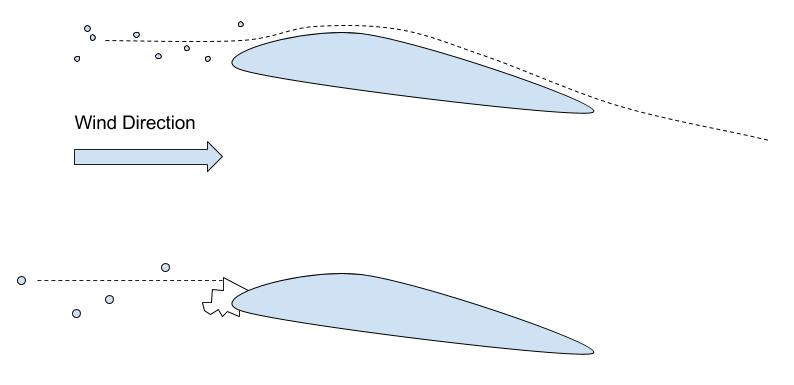
\includegraphics[width=0.6\linewidth]{figures/freezing_droplets}
\caption{Supercooled water droplets on collision course with an aerodynamic profile.}
\end{figure}


A particle’s eagerness to follow the flow or collide depends on several factors, like the flow velocity, the size of the obstacle, the density and drag coefficient of the particle. This relationship is known in fluid mechanics as the Stokes number (Stk). Small droplets or particles with Stk << 1 may continue with the airflow around the profile, while large droplets or particles with Stk >> 1 due to their inertia collide with the structure. A supercooled droplet colliding with a structure would likely freeze on the impact.

All droplets or particles approaching an obstacle are affected by the change in pressure and wind direction surrounding it, a fact which complicates measuring the concentration of particles in unaffected air. Measurement probes working by extraction of air using a mechanical air pump would expect a loss of particles with large Stokes numbers. Ideally the measuring device would affect the flow as little as possible.

Measuring particles from aircraft is complicated by the high air speed. The sample is affected by the change in pressure surrounding the aircraft and by particles hitting parts of the probe, splintering or changing direction. (ref) An instrument fixed to the ground on the other hand is affected by the wind speed relative to the ground. This means that it needs to be directed in the direction of the wind. Particles may also enter the measurement zone from different directions depending on their Stokes number, which has been shown to have a large impact on the measured liquid water content (ref).

 
%
% !TeX root = ../main.tex
% !TeX spelling = en_GB
% !TeX program = pdflatex

\chapter{Materials and Methods}
\label{chap:methods}

The methods in this chapter can be seen as the answers to research question RQ1-RQ3 from \Cref{chap:intro}. To begin with, a few different light sources and illumination angles were investigated. In section \ref{sec:discussionstarting}, the lighting alternatives that were considered, are described. It was settled that a shadowgraph system with background illumination from an \gls{led} was to be used. The experimental setup was tested using different water droplet generators and a test target consisting of micrometer sized lines and dots. Analyzing the optical system and testing different segmentation algorithms, we found a simple way to define the sample volume for each individual droplet. To test the ability of measuring concentration we needed to build a weather protected prototype that could be used in parallell with a second instrument. The prototype needed to be fully automatic, able to analyze images in real time 24 hours a day for several months and store the results in a compressed format. To calibrate the size measurement and the measurement range, the previously mentioned dots of different sizes were used. The size measurement was also verified using distributions polymer microspheres, applied by blowing compressed air through a glass dispenser.

\section{The Shadowgraph System}

The instrument is a shadowgraph system using a monochrome \gls{cmos} camera with a 4x magnifying telecentric lens and a \gls{led} with a collimating lens illuminating the background. \Cref{fig:shadowprinc} shows a sketch of the system. The system was first tested in the experimental setup seen in \Cref{fig:experimental}. 

\begin{figure}[ht]
\centering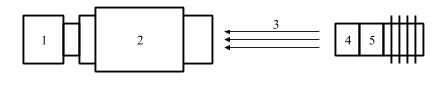
\includegraphics[width=0.75\linewidth]{./figures/shadowprinc.jpg}
\caption{Principle of shadowgraphy. 1. Camera. 2. Telecentric lens. 3. Parallell focused light beam. 4. Collimating lens. 5. \gls{led}.}
\label{fig:shadowprinc}
\end{figure}

The blue \gls{led}, shown to the right in \Cref{fig:experimental}, was initially powered by a SignaTech Strobe Controller from Advanced Illumination. The SignaTech Controller can produce up to 4A at 100V. For the prototype instrument, another current driver, the Picolas LDP-V 10-70 was chosen. This driver can produce short 12A pulses. For controlling the pulse length, a microcontroller is used. 

\begin{figure}[ht]
\centering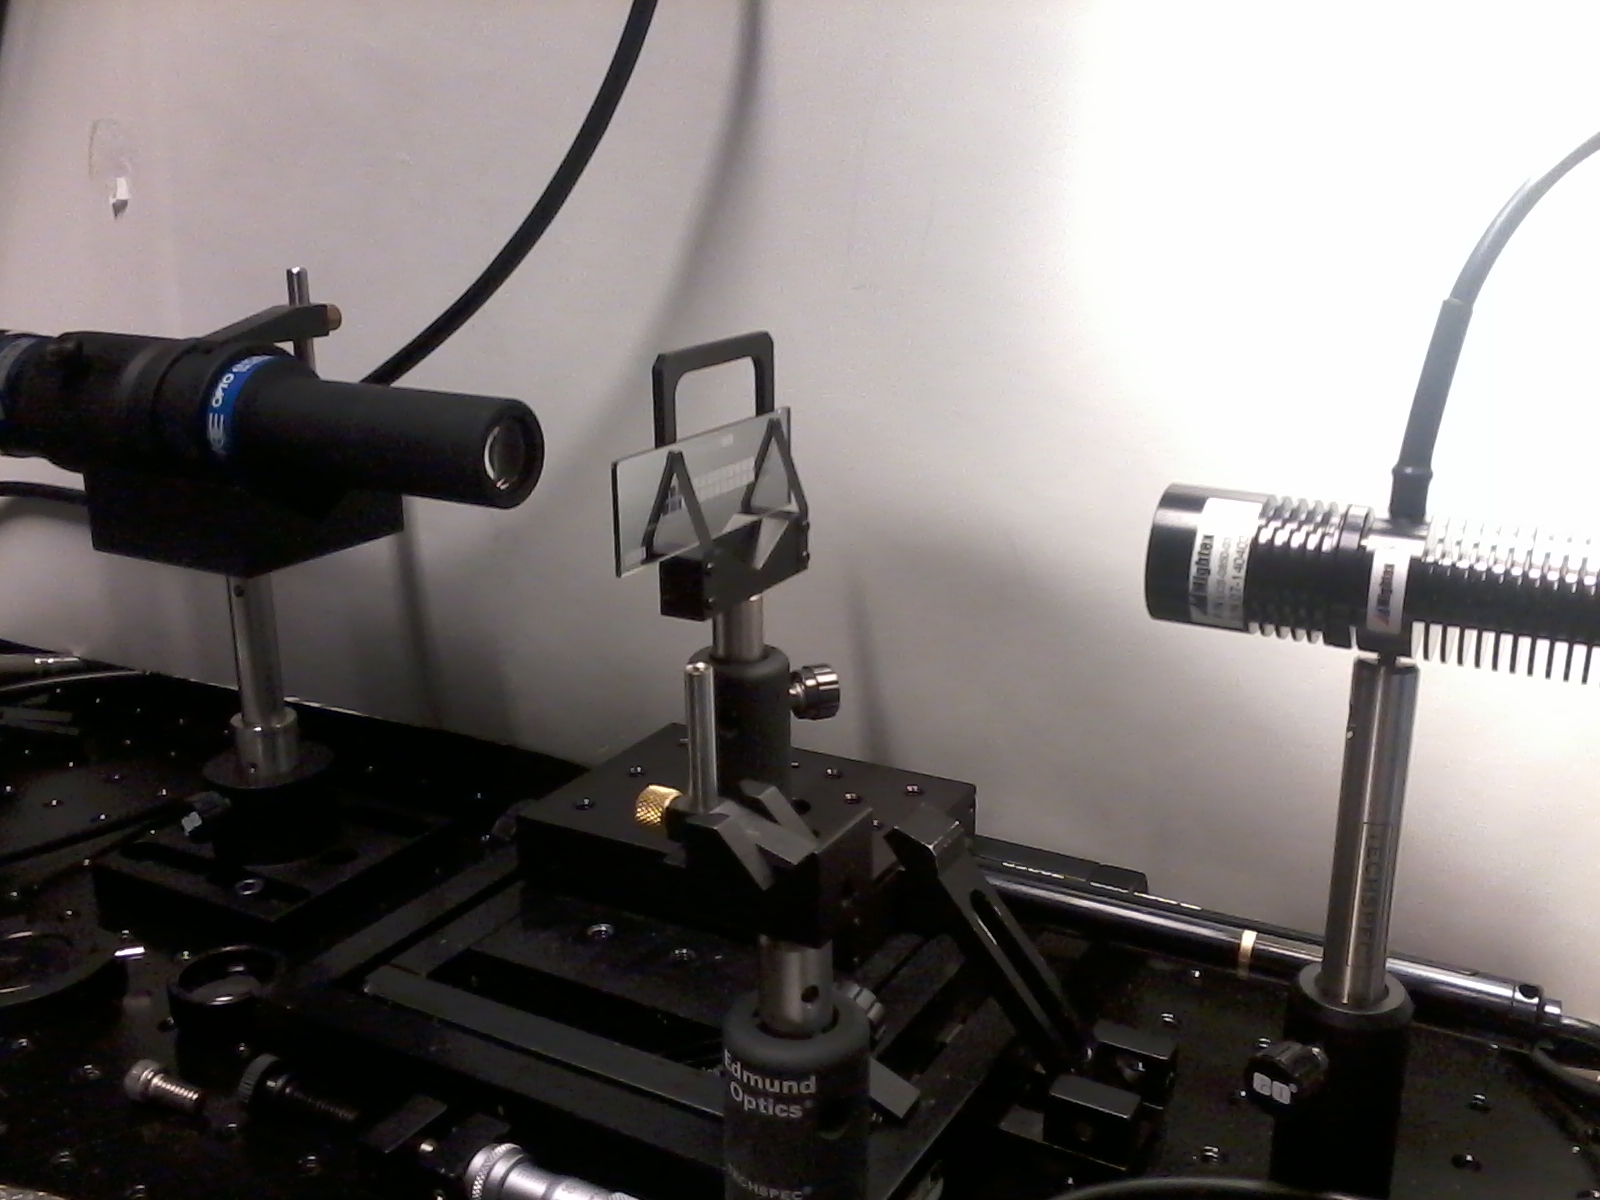
\includegraphics[width=0.75\linewidth]{figures/Foto0169}
\caption{The experimental setup with a dot micrometer scale as test object mounted on a translation stage.}
\label{fig:experimental}
\end{figure}

The complete system was mounted in a weather proof shell using two standard camera housings and a separate box for the analyzing computer and power supply. \Cref{fig:housings} shows the system mounted in weather proof camera housings. 

\begin{figure}[ht]
\centering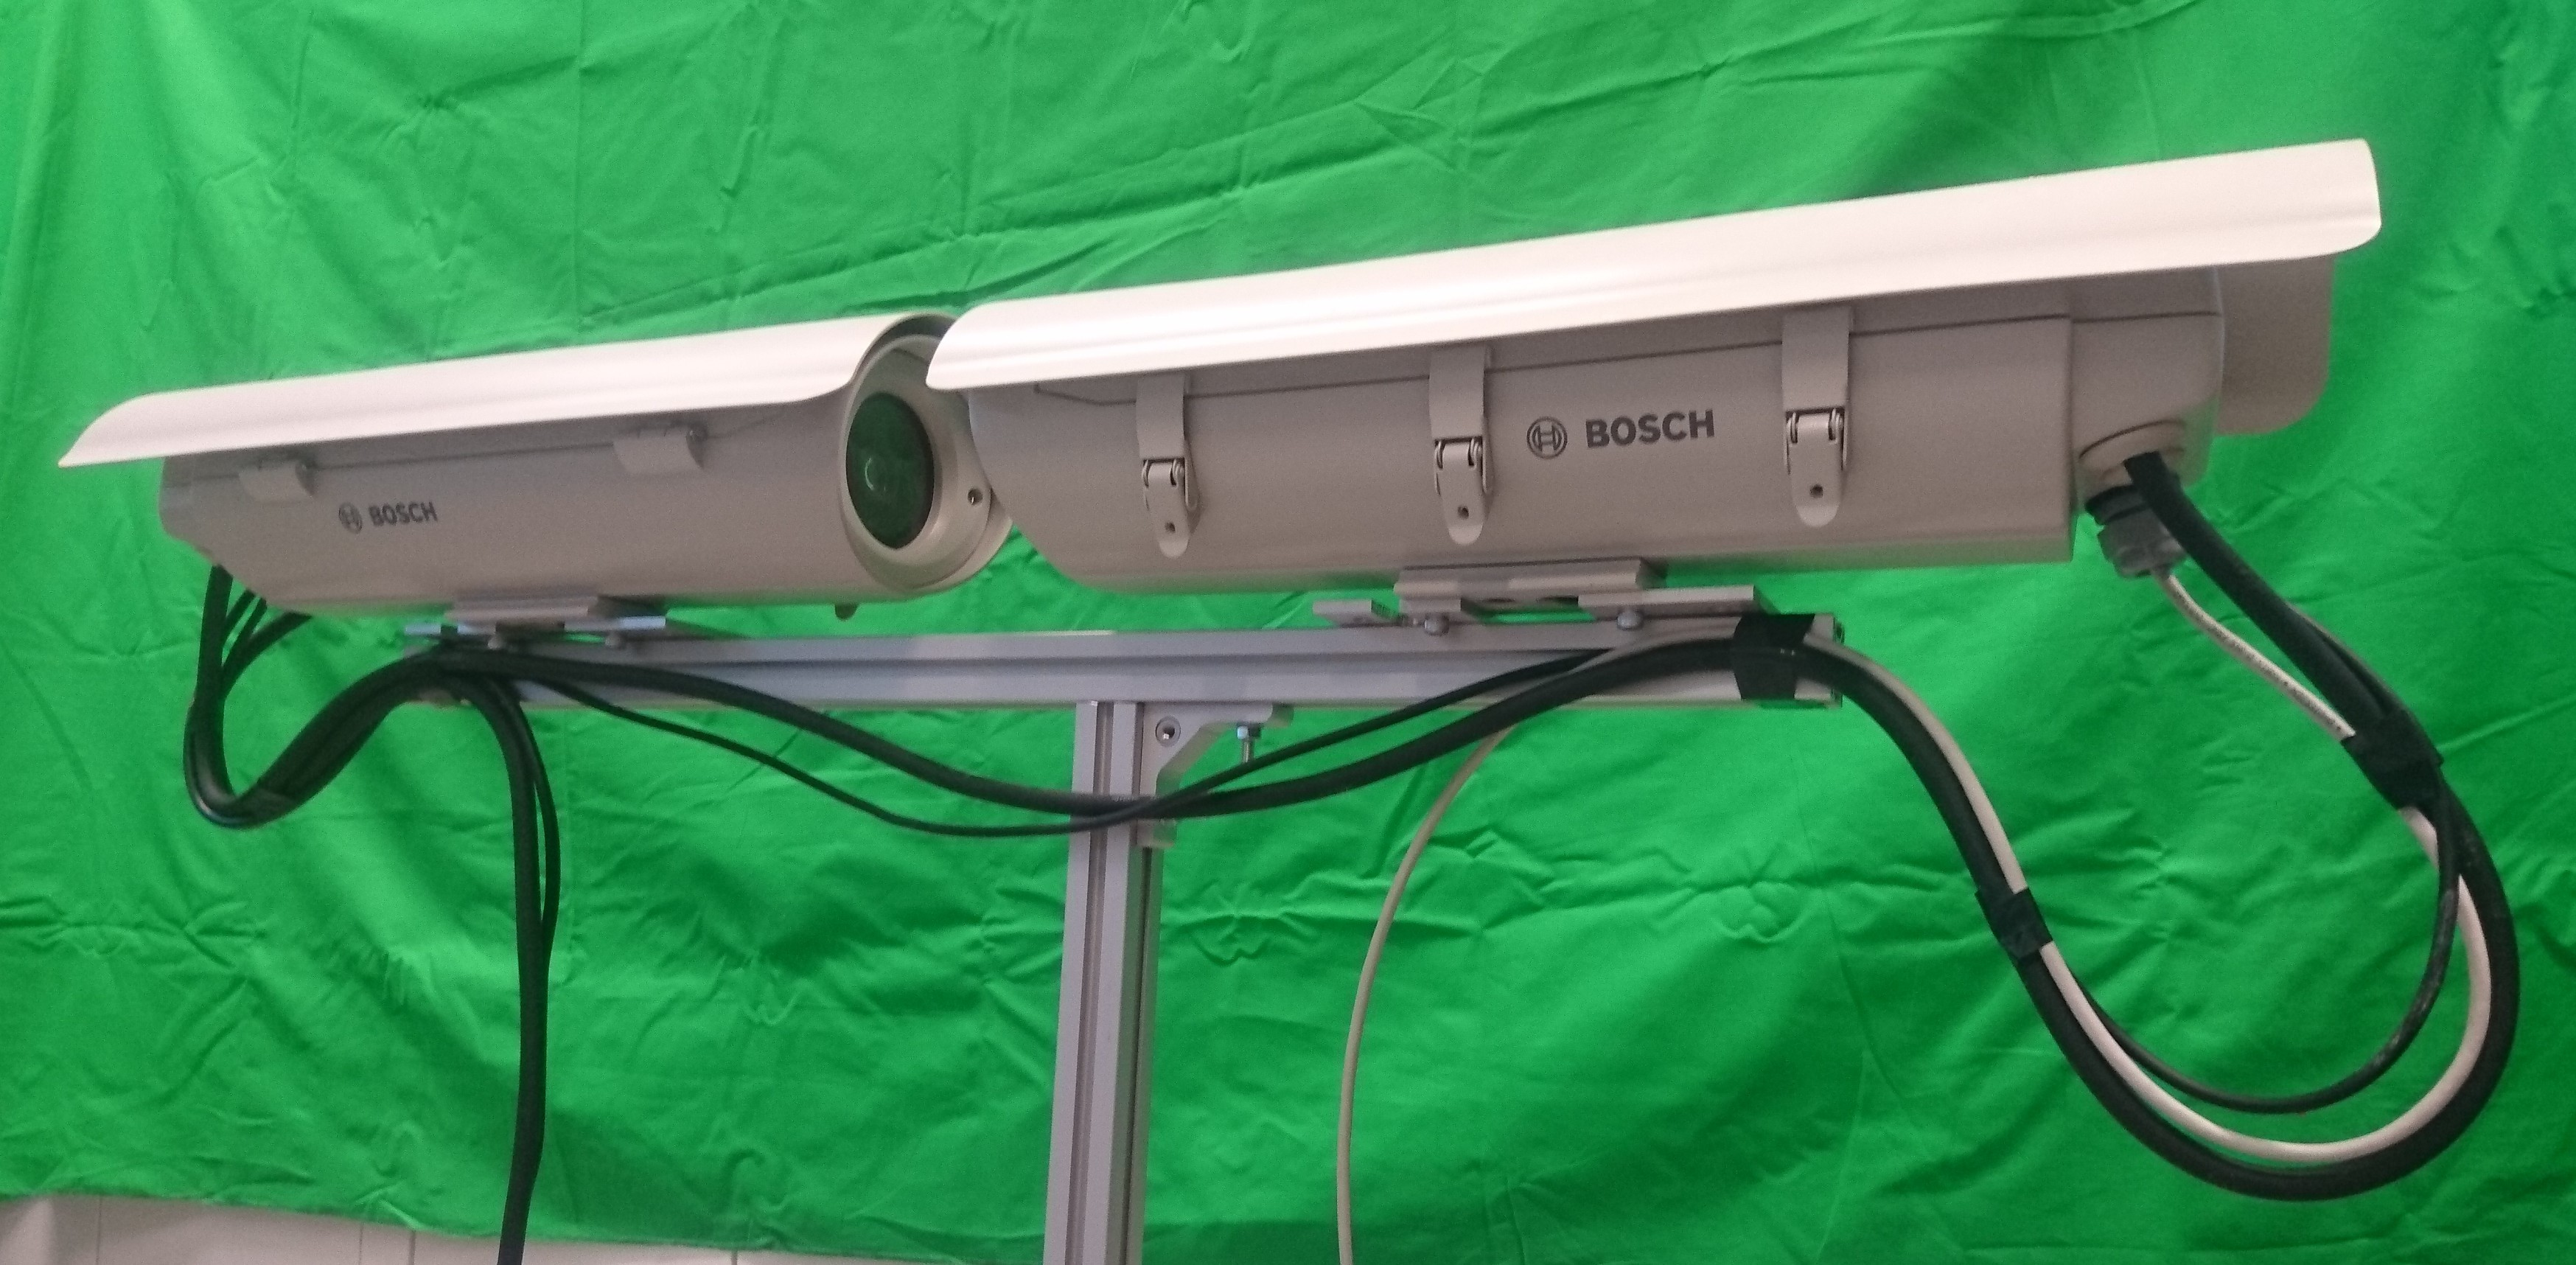
\includegraphics[width=0.75\linewidth]{figures/cam_housings}
\caption{The illumination and detector is mounted inside two Bosch camera housings facing each other with heating inside the housings and on the front glass.}
\label{fig:housings}
\end{figure}

\section{Overview and Process}
\label{sec:overview}

\begin{figure}[ht]
\centering\includegraphics[width=0.75\linewidth]{figures/El_interfaces}
\caption{Electrical interfaces and system overview.}
\label{fig:el_if}
\end{figure}

A stage micrometer scale was used for characterization of the system and simulation of water droplets. This characterization holds true given that the optical silhouette of a droplet is comparable to a dot of equal diameter printed on a silicon glass. It is not a new concept and has been proved experimentally by comparing beads of glass and water droplets of known sizes \cite{koro1991,koro1998}. Light passing a transparent sphere is affected by its refraction, reflection, diffraction and absorption. Of these four components, the shadow will be defined mainly by the diffracted, as long as the distance between the sphere and the lens is much greater than the sphere's diameter \cite{koro1991,wend2013}.

The design using a weakly collimated \gls{led} that illuminates an area slightly larger than the field of view makes the system quite insensitive to misalignment of the camera and the light source. Temporal or permanent changes in light intensity caused by a minor misalignment are automatically compensated for by continuous measurement of the total exposure level. If the level of exposure is increasing or decreasing, the length of the light pulse is changed correspondingly. The light intensity can also be affected by dirt on the front glass of the housings. 

Since many images do not contain any droplets at all, we increase the processing speed by sorting out the images that do not contain any interesting information. This is done by constructing an average image from 20 images. All new images are compared with this average, and if any pixel differs from the average, by more than a specific value that is significantly higher than the noise level, the image is analyzed. The average image is re-constructed periodically.

Spatial dissimilarities in the light intensity that are not caused by noise are compensated for by calculating the local average intensity of the background around each measured droplet. This way, a variable threshold \cite{gonz2002} is constructed.The size of a droplet is then based on the intensity dip caused by the shadow compared with its local background.

\begin{figure}[ht]
\centering\includegraphics[width=0.75\linewidth]{figures/Img_proc}
\caption{Flowchart illustrating the method of image processing step by step.}
\label{fig:img_proc}
\end{figure}

\section{Image Segmentation}
\label{imgsegment}

If the image contains an object detected by the thresholding, the sample volume is calculated for each droplet individually depending on its size. By using a Laplacian of Gaussian \cite{marr1980, gonz2002} edge detection and a suitable threshold, we can create closed curves around objects where the edge is in or near focus. Other edge detection operators like Roberts, Prewitt, Sobel \cite{gonz2002} and Canny \cite{canny1986} did not seem to give the same consistant performance in different lighting conditions. The objects that create closed curves, selected by a boundary fill function, are said to be within the measuring range. The measuring range together with the field of view defines the sampling volume. The measurement volume is described in Paper I. Since the Laplacian of Gaussian can be seen as value of the second derivative of the edge gradient, it is also used together with the diameter to calculate the true size of the droplet. This is described in Paper II.

\subsection{Exposure Check and Flash Intensity Adjustment}

Let $I_{i,j}$ denote the two-dimensional image captured by the camera. The mean value $\overline{i}$ of all pixels in the image $I_{i,j}$ gives an estimation of the exposure level in the whole image. 

The flash duration is adjusted automatically by the microcontroller at each exposure to keep the exposure level between a low and a high threshold, $th_L$ and $th_H$. The duration is changed in steps of 13 ns corresponding to one clock cycle of the microcontroller. If $\overline{i} > th_L$ and $\overline{i} < th_H$ the image is analyzed. If $\overline{i} \geq th_H$ the flash duration is decreased by steps of 12 ns. If $\overline{i} \leq th_L$ the flash duration is increased. The total flash duration is approximately 250 ns. Here $th_L$ is set to 0.7 and $th_H$ is set to 0.8 in a normalized (0,1) dynamic range.

\subsection{Edge Detection and Edge Sharpness}

To detect the intensity changes created by the shadow of a water droplet, an image is processed using the Laplacian of Gaussian (LoG) described by Marr and Hildreth \cite{marr1980}. The method works by looking for zero crossings in the image resulting from calculating $\nabla^2 G\left(x,y\right) * I\left(x,y\right)$. $G\left(x,y\right)$ is a two-dimensional Gaussian distribution with standard deviation σ and $\nabla^2$ is the Laplacian operator, defined as the divergence of the gradient in two dimensions.
\begin{equation}
G\left(x,y\right) = \frac{1}{\pi \sigma^2} e^{-\frac{x^2+y^2}{2\sigma^2}}
\end{equation}
\begin{equation}
\nabla^2=\nabla\cdot\nabla=\frac{\delta^2}{\delta x^2} + \frac{\delta^2}{\delta y^2}
\end{equation}
We implement a discrete approximation to $\nabla^2 G\left(x,y\right) \approx \nabla^2 G_{i,j}$ as a 13x13 sized convolution kernel.
\begin{equation}
\nabla^2 G_{i,j} = -\frac{1}{\pi \sigma^4} \left(1 - \frac{i^2+j^2}{2\sigma^2} \right) e^{-\frac{i^2+j^2}{2\sigma^2}}
\end{equation}
By applying the convolution to the normalized image $I_{i,j}$ we get the image $P_{i,j}$.
\begin{equation}
P_{i,j}=\nabla^2 G_{i,j} * I_{i,j}
\end{equation}
$P_{i,j}$ is thus a matrix that contains the second order derivative of the image $I_{i,j}$. 
A spherical object will result in an edge where the intensity change is similar around a spherical object, but dependent on the distance from the optimal focus. Assuming the Gaussian of the image I is twice differentiable at any point $(i,j)$, the maximum (or minimum) of the second derivative includes the amplitude of the first derivative at the point where the second derivative is equal to zero, i.e. where the edge is strongest. This can be intuitively understood; when the edge is sharper, the gradient, or first derivative value, is larger. And if the gradient value is larger, the rate of change, i.e. the second derivative, needs to be larger at each side of the edge. Therefore, we store a value of the maximum second derivate, $max(P_{i,j}$), around each analyzed object and use this as a measure of the edge sharpness. This value in turn is used as input to a calibration function. 
We also construct a new binary image $Q$ in which the pixel value $Q_{i,j}=1$ if any of $|P_{i+1,j}-P_{i,j} |,|P_{i-1,j}-P_{i,j} |,|P_{i,j+1}-P_{i,j} |,|P_{i,j-1}-P_{i,j} |>th$, where $th=0.002$. $Q_{i,j}=0$ elsewhere. th is the gradient of the second derivative at the point where the second derivative is zero, i.e. on the edge. Particles are found by searching for closed contours in this binary image.

\subsection{Comparing Transparent Microspheres and Dots}

A spherical lens scatters almost all the incident light in different directions, leaving only a bright spot in the middle where the light is transferred directly through. For larger particles in focus, this bright spot can result in a second circular closed contour inside the outer edge. 

Small water droplets can be seen as transparent microspheres. The composition changes the refractive index, but this has little effect on the shadow. The outer contour is the same following the same reasoning as dots used for calibration in Paper I. Diffraction patterns depend on the wavelength of the light and the size of the sphere. The resolution of the constructed system is not high enough for these patterns to be visible.

By using a flood-fill function on the binary image containing the detected contour, starting at a point at a minimum distance from an object, the edge of the filled area will border to the outer contour. This makes it possible to select the outer closed contours of possible particles.

\subsection{Removing the Center Bright Spot}

The center bright spot will make the shadow of a transparent sphere brighter in average than a solid dot. This will have an impact on the size calculation, since the size calculation is based on the shadow impact and the calibration is done using solid dots. Therefore, we apply a mask on the image before calculating the size of the shadow. The mask is done by replacing all the centermost pixels in the shape of a circular disc with the intensity of the darkest pixel in the spot. The diameter of the masked disc is the arc length of the edge contour divided by $\pi$. The bright spot is measured by calculating the difference between the least value and the center pixel. Only particles with a difference greater than 0.1 (ten percent) will have the mask applied

\subsection{Measuring Roundness}
\label{met:roundness}
There may be clogs of small microspheres or dust in the samples that are measured. Microspheres, or small water droplets are close to spherical. We try to exclude all objects that the program finds that are not circular. After the detection of object edges, we measure the roundness of each object. A measure of the mean square roundness deviation similar to the one described by ISO \cite{iso12181} can be achieved by calculating the quote between the area of the contour and the square of the total arc length. See (\ref{eq:5}).
\begin{equation}
roundness = 4\pi \frac{A_{contour}}{arcLength^2}
\label{eq:5}
\end{equation}
$A_{contour}$ is the pixel area of the filled contour and $arcLength$ is the perimeter of the measured closed contour. In the calibration and field measurements described, an object is only considered spherical if $roundness \geq 0.85$.

\section{Light Source}

Although water is a good absorber of electromagnetic radiation in most spectral wavelenghts except for the visible, the volume of water droplets is too small for the absorbtion to be measurable. In visible light, the water droplet can be regarded as a spherical lens with a very short focal length, thus spreading most of the light in diverging directions. Since the camera used is designed for both visible and near infrared light, we tested and compared two different wavelenghts, 455 nm and 850 nm using the same optical setup. The shorter wavelength gave sharper images and higher \gls{snr}.

\begin{figure}
\centering
\begin{minipage}{.5\textwidth}
  \centering
  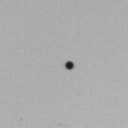
\includegraphics[width=.6\linewidth]{figures/compare455nmdot}
  %\caption{A subfigure}
  %\label{fig:compare455nmdot}
\end{minipage}%
\begin{minipage}{.5\textwidth}
  \centering
  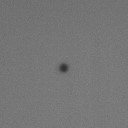
\includegraphics[width=.6\linewidth]{figures/compare850nmdot}
  %\caption{A subfigure}
  %\label{fig:compare850nmdot}
\end{minipage}
\caption{The same dot viewed with different background light: 455 nm (left) and 850 nm (right).}
\label{fig:comparedots}
\end{figure}

\subsection{Laser Light}

For conventional imaging of small particles the coherence of laser light mainly causes problems as diffraction patterns will be strong and visible. Therefore this was only briefly investigated. In section \ref{sec:discussionlaser} there is a discussion of the result from this investigation.

\subsection{Ambient Light}

In daylight, there is always some ambient light. Although the camera is never aimed direclty at the sun and has a telecentric lens, we wanted to be sure that this light would not affect the measurement. For an indication the amount of ambient light, the system was tested in daylight, using a fog generator in front of the lens to reflect light into the lens. 

\section{Image Noise}

We had an idea that it should be possible to measure the signal to noise relation, if the shadow image of the droplet represents the signal. In theory, the \gls{snr} could be used as an input to the size or concentration calculation, to increase the accuracy of the measurement. 

An estimation of the image noise in the whole image was done by making a number of images using only the background illumination. The standard deviation was calculated in each pixel of the 2048x2048 sized image, resulting in an average variation coefficient of about nine percent.

A function was created that calculates the noise level locally around each analyzed droplet image. Assuming that the area surrounding a droplet is evenly illuminated, the SNR can be estimated for each droplet $j$, as the relation between the signal and the ambient noise. The signal is the light amplitude, A$_j$, and the noise is the standard deviation of the surrounding noise, $\sigma_j$. See (\ref{eq:snrcalc}) and \Cref{fig:snrcalc}.

\begin{equation}
snr_j = 20 log \frac{\text{A}_j}{\sigma_j}
\label{eq:snrcalc}
\end{equation}

\begin{figure}%[ht]
\centering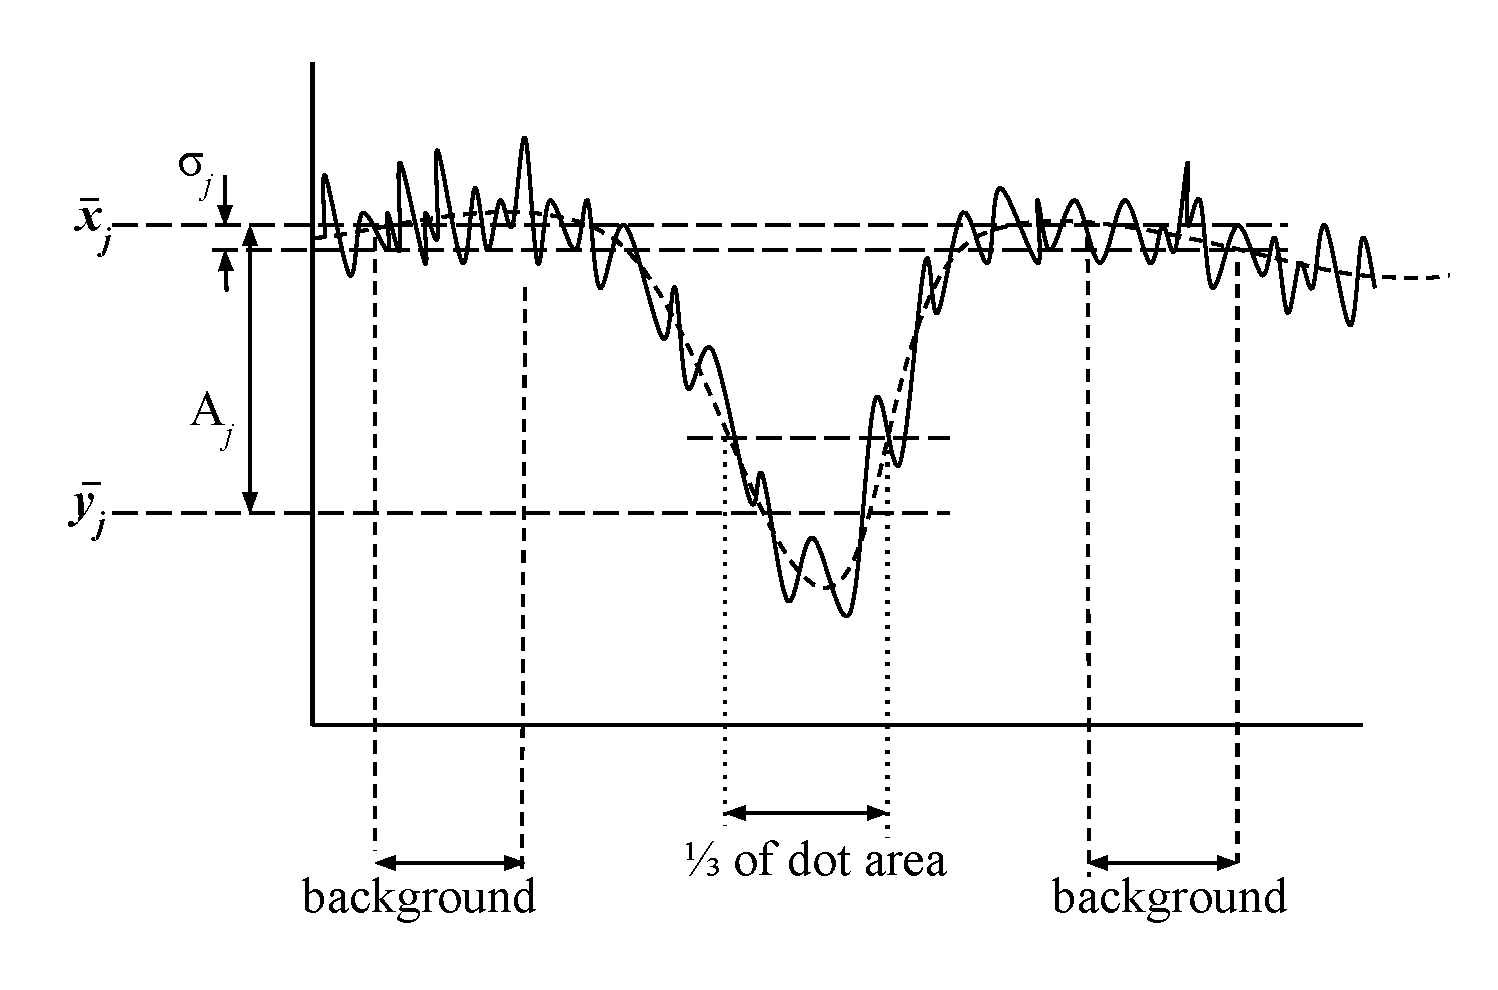
\includegraphics[width=0.75\linewidth]{figures/snrcalc}
\caption{Calculation of the SNR. $\overline{y}_j$ is determined by calculating the average of the darkest third of all pixels inside the edge detected dot.}
\label{fig:snrcalc}
\end{figure}

%\subsection{Exposure Energy Measurement}
%
%This measurement was done to get an idea about the theoretical minimum amount of energy required for each image. In practice, the light from the collimated LED used will be spread so that only a small part of the total emitted energy actually reaches the sensor. The area in view is about 8 times smaller than the illuminated area of the collimated LED, which was measured to about 8x8 mm. Some of the light energy will be absorbed in the telecentric lens.
%
%The light energy required for good exposure was investigated using eight gain setting levels. A pulsed signal was used, 3-10 μs long, with 9-36 kHz frequency. To minimize the thermal effect of the heated glass and the ambient light, the power was measured immediately before and after start and stop. The pulse length was measured using a semiconductor light sensor connected to an oscilloscope. The result is discussed in section \ref{sec:expmeasurement}.


\section{Calibration and Validation of the Calibration}

Because of the diffraction, the edge of an object is difficult to measure directly by thresholds, even if the coherence length of the light is small and the object is in focus. The edge will apprear blurry. For objects out of focus, the blurring will increase even more. Therefore the size measurement is calibrated by both measured diameter and a value of the edge sharpness, or gradient.

Also the measuring range needs to be calibrated. The measuring range is here defined as the distance in which the edge detection by Laplacian of Gaussian operator and a threshold makes a closed curve in the resulting binary image. This will be different especially for smaller objects.

The system was calibrated using a stage micrometer scale with 13 circular dots printed in chrome on a silicon glass. The dots range from 2 to 100 μm in diameter. Each dot was moved linearly in steps of one micrometer in the direction orthogonal to the lenses, thus creating a function where the gradient of the edge depends on the distance from optimum focus. A threshold on the second derivative gradient strength limits the measured particles to be within a specific measuring range. The threshold should be selected carefully. If the value of the threshold is too low, there will be many false edges in the image. If it is too high, the measuring range will be too small. The difference between two different thresholds, 0.002 and 0.005 is illustrated by \Cref{fig:measrangevslogth}. The lower threshold was used in the following measurements.

\begin{figure}[ht]
\centering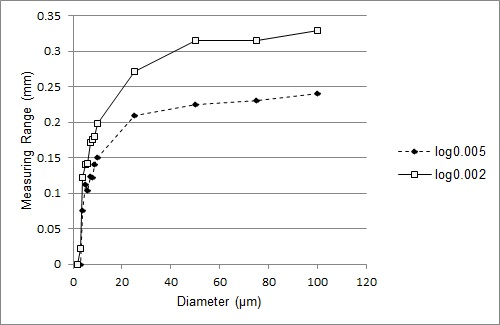
\includegraphics[width=0.75\linewidth]{figures/meas_range_vs_log_th}
\caption{Measuring range (mm) vs. diameter for two different thresholds (0.005 and 0.002).}
\label{fig:measrangevslogth}
\end{figure}

The edge sharpness will affect the position of the edge and the measured shadow slightly. We use the maximum value of the second derivative $P_{i,j}$ for each droplet as a measure of the edge sharpness and include this in the calibration functions, together with the diameter measured from the shadow intensity.

Two second degree approximation surfaces, (\ref{eq:z1}) and (\ref{eq:z2}), are calculated using the “fit” command in Matlab. $z_1$ approximates dot diameters from 2 to 10 micrometers and $z_2$ diameters from 10 to 100 micrometers. x is the maximum second derivative, $d^M$ is the diameter measured from the shadow intensity, $p_{xx}$ and $q_{xx}$ are constants.

\begin{equation} \label{eq:z1}
z_1=p_{00}+p_{10} x+p_{01} d^M+p_{20} x^2+p_{11} xd^M+p_{02} {(d^M)}^2
\end{equation}
\begin{equation} \label{eq:z2}
z_2=q_{00}+q_{10} x+q_{01} d^M+q_{20} x^2+q_{11} xd^M+q_{02} {(d^M)}^2
\end{equation}
By measuring the calibrated microspheres a validation can be made with the expected diameter. 

\subsection{Verification of Dot Size}

The dots on the micrometer scale were measured visually using a Leica microscope connected to a digital camera. This was done to find accurate values of the diameter of the dots to use in the calibration. An example image that was measured can be seen in \Cref{fig:50umdot40x}.

\begin{figure}[ht]
\centering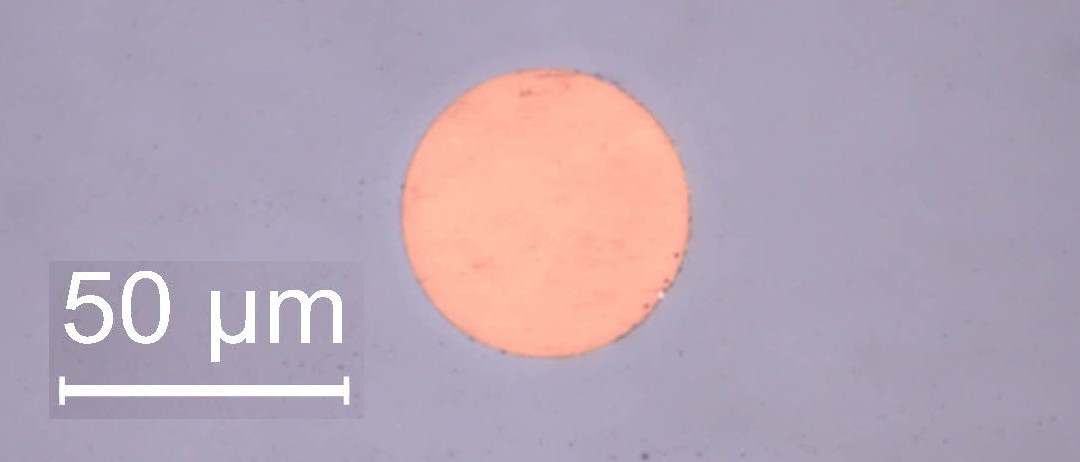
\includegraphics[width=0.75\linewidth]{./figures/50umdot40x.jpg}
\caption{The 50 micrometer dot with front illumination imaged using 40x magnifying lens.}
\label{fig:50umdot40x}
\end{figure}

This measurement was done using lenses with two different magnifications: 40x and 100x. All the dots average diameters, except the 100 µm dot were found to be within $\pm$0.2 $\mu$m of their nominal diameter. They are not all perfectly round, but the size accuracy should be good enough to use as calibration reference. The result from this measurement is presented in \Cref{tab:ref_meas}.

\begin{table}[ht]
\centering
\begin{tabular}{p{0.2\linewidth} p{0.2\linewidth} p{0.2\linewidth} p{0.2\linewidth}}
\hline
\textbf{Nominal Diameter} & \textbf{Excentricity} & \textbf{Diam. 40x} & \textbf{Diam. 100x} \\
\hline
5 & 0.2 & 5 & 4.8 \\
6 & 0.6 & 5.8 & 5.8 \\
7 & 0 & 7 & 6.6 \\
8 & 0 & 8 & 7.9 \\
9 & 0 & 9 & 8.8 \\
10 & 0 & 10.1 & 9.8 \\
25 & 0 & 24.9 & 24.7 \\
50 & 0.4 & 50.1 & 49.8 \\
75 & 0.2 & 75.2 & 74.8 \\
100 & 2.5 & 100 & 98.7 \\
\hline
\end{tabular}
\caption{Micro dot verification measurement. All values are in µm. Here, eccentricity is the maximum difference in µm between the smallest and the largest measured diameter.}
\label{tab:ref_meas}
\end{table}



\section{The Fog Chamber}

Natural fogs tend to not coincide with when we are ready to test. The fog chamber was needed to create a test environment for the instrument. 

The constructed chamber has a frame made of 30 mm aluminum profiles, fitted with transparent 6 mm polycarbonate walls on all sides using rubber sealing strips. The droplets are produced using an ultrasonic fog generator pushing the droplets to the chamber through a flexible tube approximately 30 mm in diameter and 500 mm long. Next to the fog inlet, there is a dry air inlet with a speed adjustable fan. On the back of the chamber there is a similar-sized outlet for air and moisture. See \Cref{fig:fogchamber}.

\begin{figure}[ht]
\centering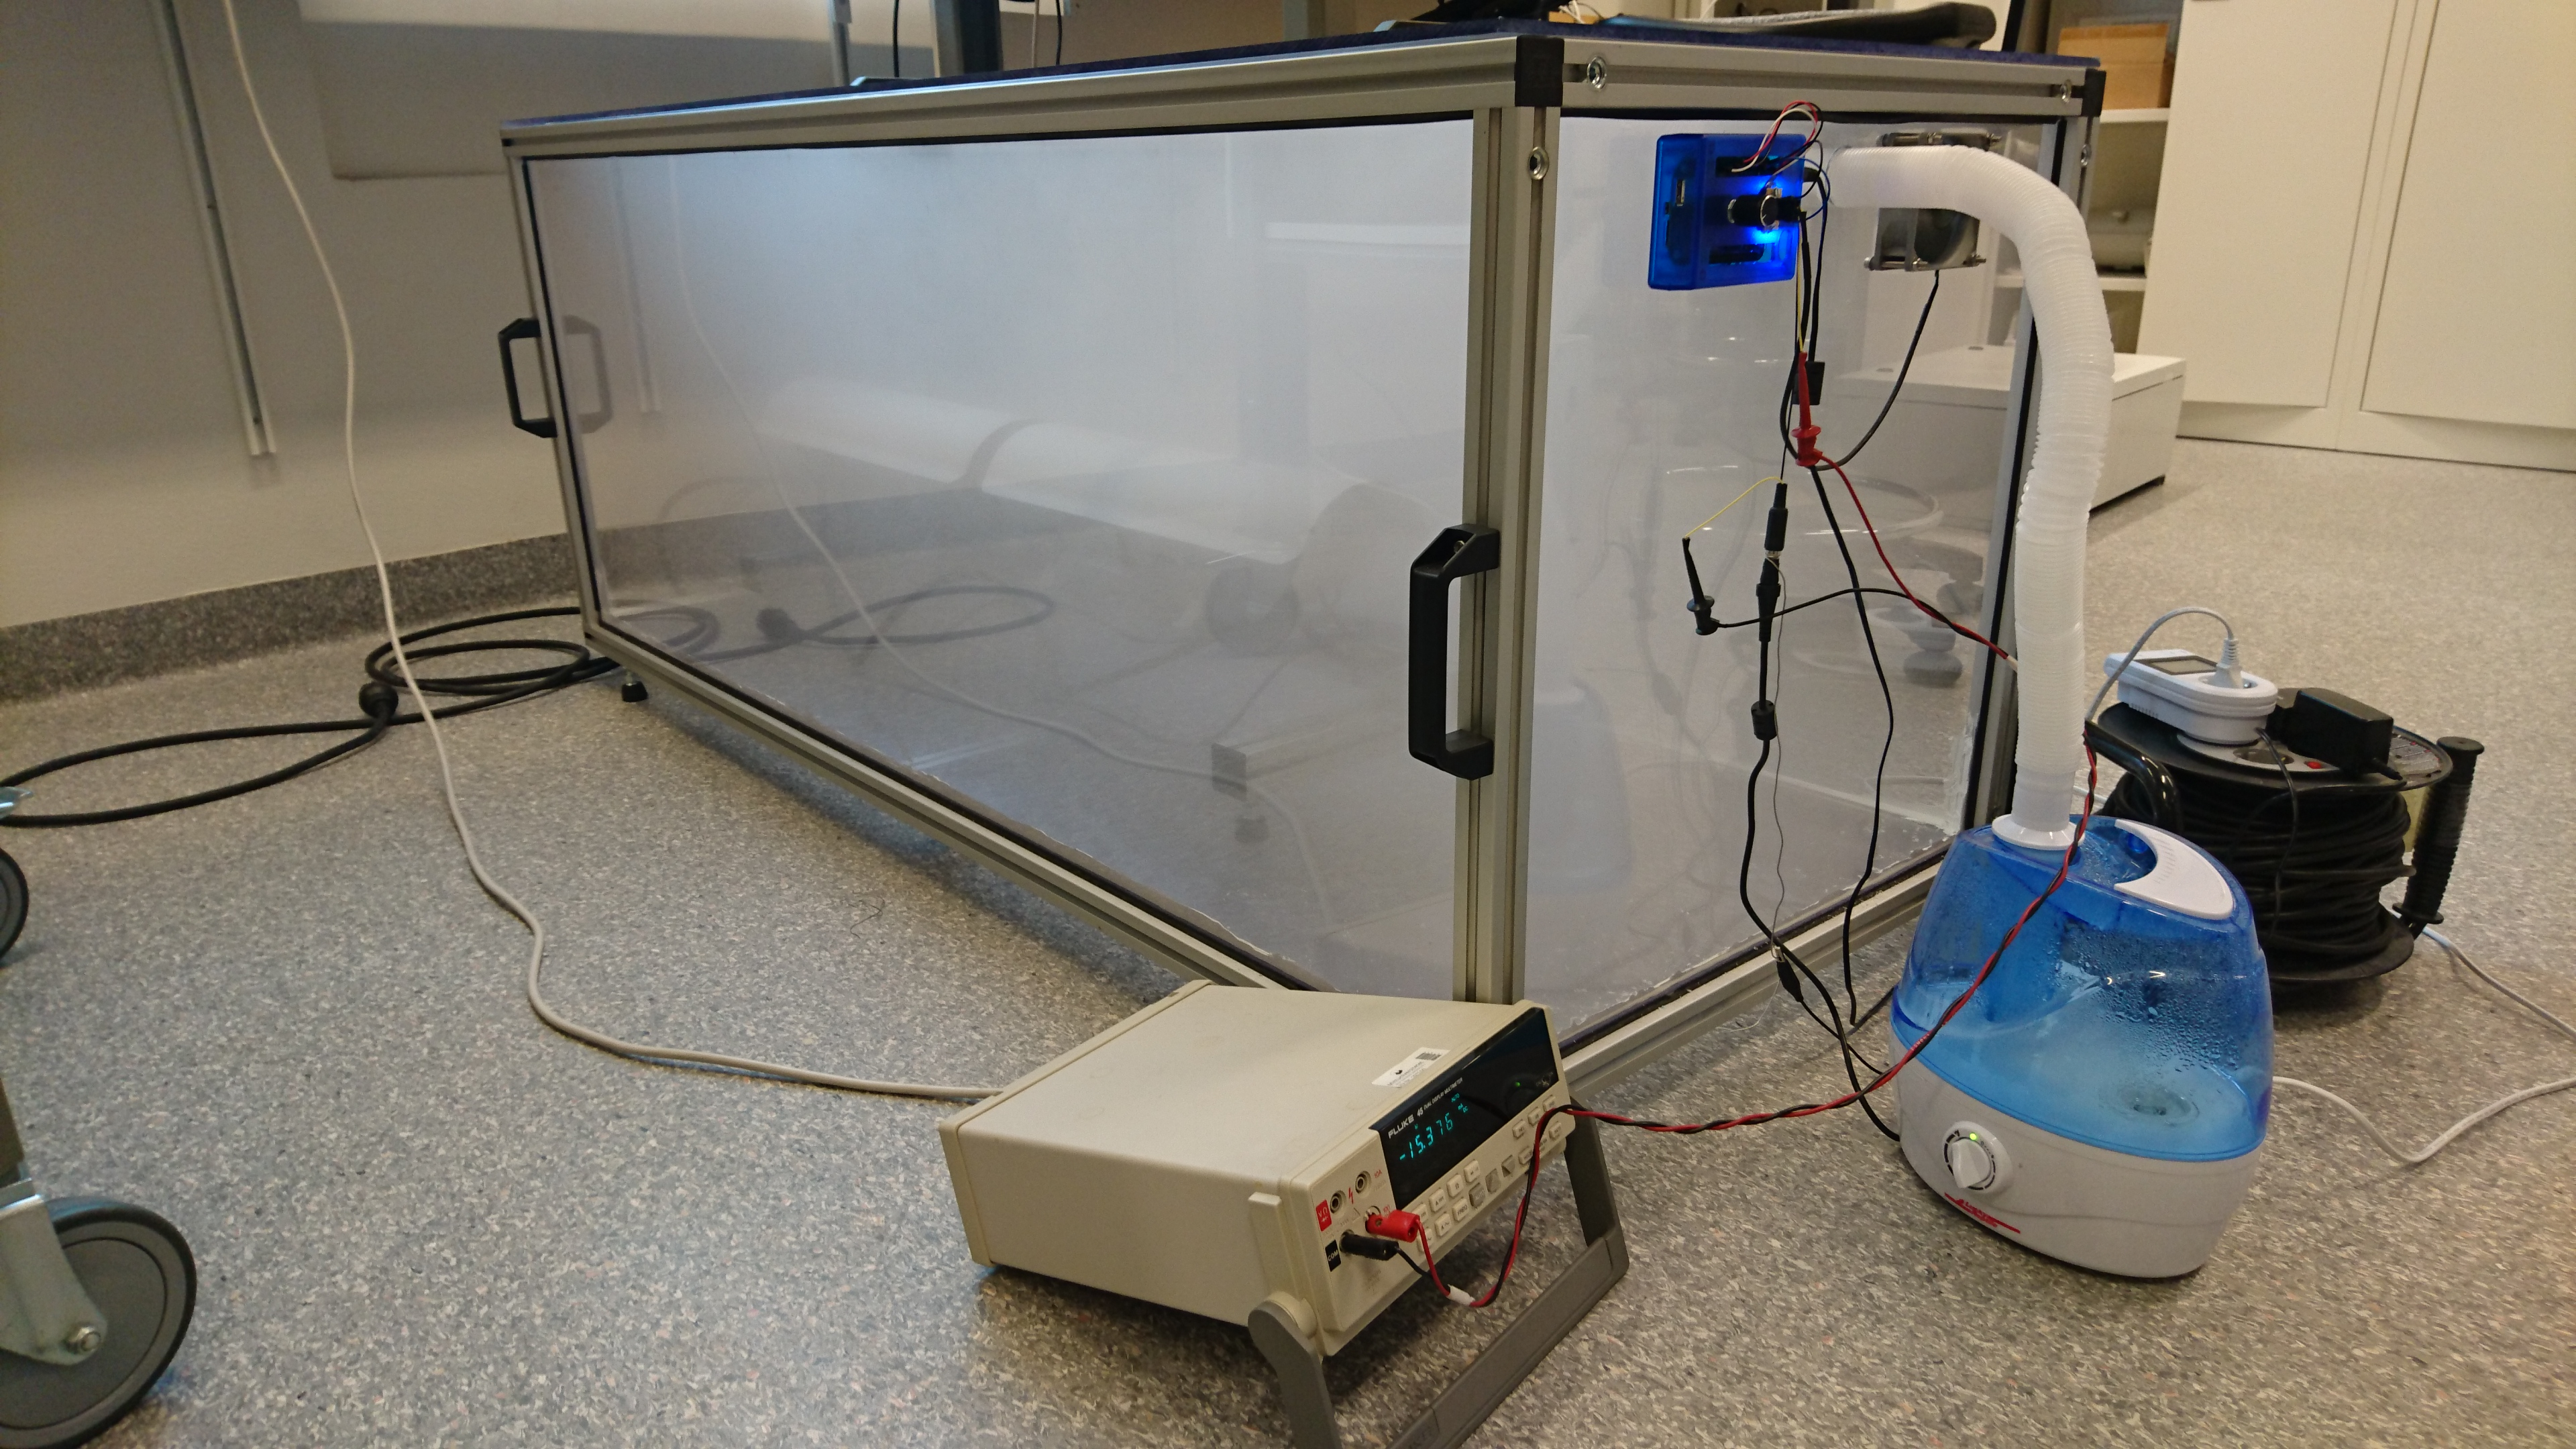
\includegraphics[width=0.75\linewidth]{figures/DSC_0103}
\caption{Fog chamber with connected droplet generator (blue container) and a multimeter used for fan power measurement. A Beaglebone Black microcontroller (blue box) is used for fan speed regulation.}
\label{fig:fogchamber}
\end{figure}
 
Unfortunately, we could not fit a second instrument in the fog chamber for verification of the \gls{lwc}. The \gls{cdp} requires an airflow with a known speed to be able to calculate the particle concentration. The fog chamber worked very well as a functional test and a verification of the instrument’s water ingress resistance.

\section{The Klövsjö Installation}

\Cref{fig:installation1} shows a complete installation of the DII and the \gls{cdp} at the Klövjö mountain. The two camera houses of the DII are placed on the top, and the smaller \gls{cdp} right underneath. The Lambrecht Eolos weather sensor is placed to the far left, mounted on an horizontal boom. In the middle, to the right of the Eolos, the mobile communication antenna is located. The top of the shortened lattice mast can be seen just below the center. Behind the mast, the top of the box containing the DII processing computer, the \gls{cdp} data collection computer, and the communications router can be seen. The whole installation is about five meters high. An electric servomotor mounted at the base of the pole inside the lattice mast rotates the two instruments automatically to follow the horizontal direction of the wind. 

\Cref{fig:installation3} shows a mix of ice and snow on the front side of the installation.

\begin{figure}[ht]
\centering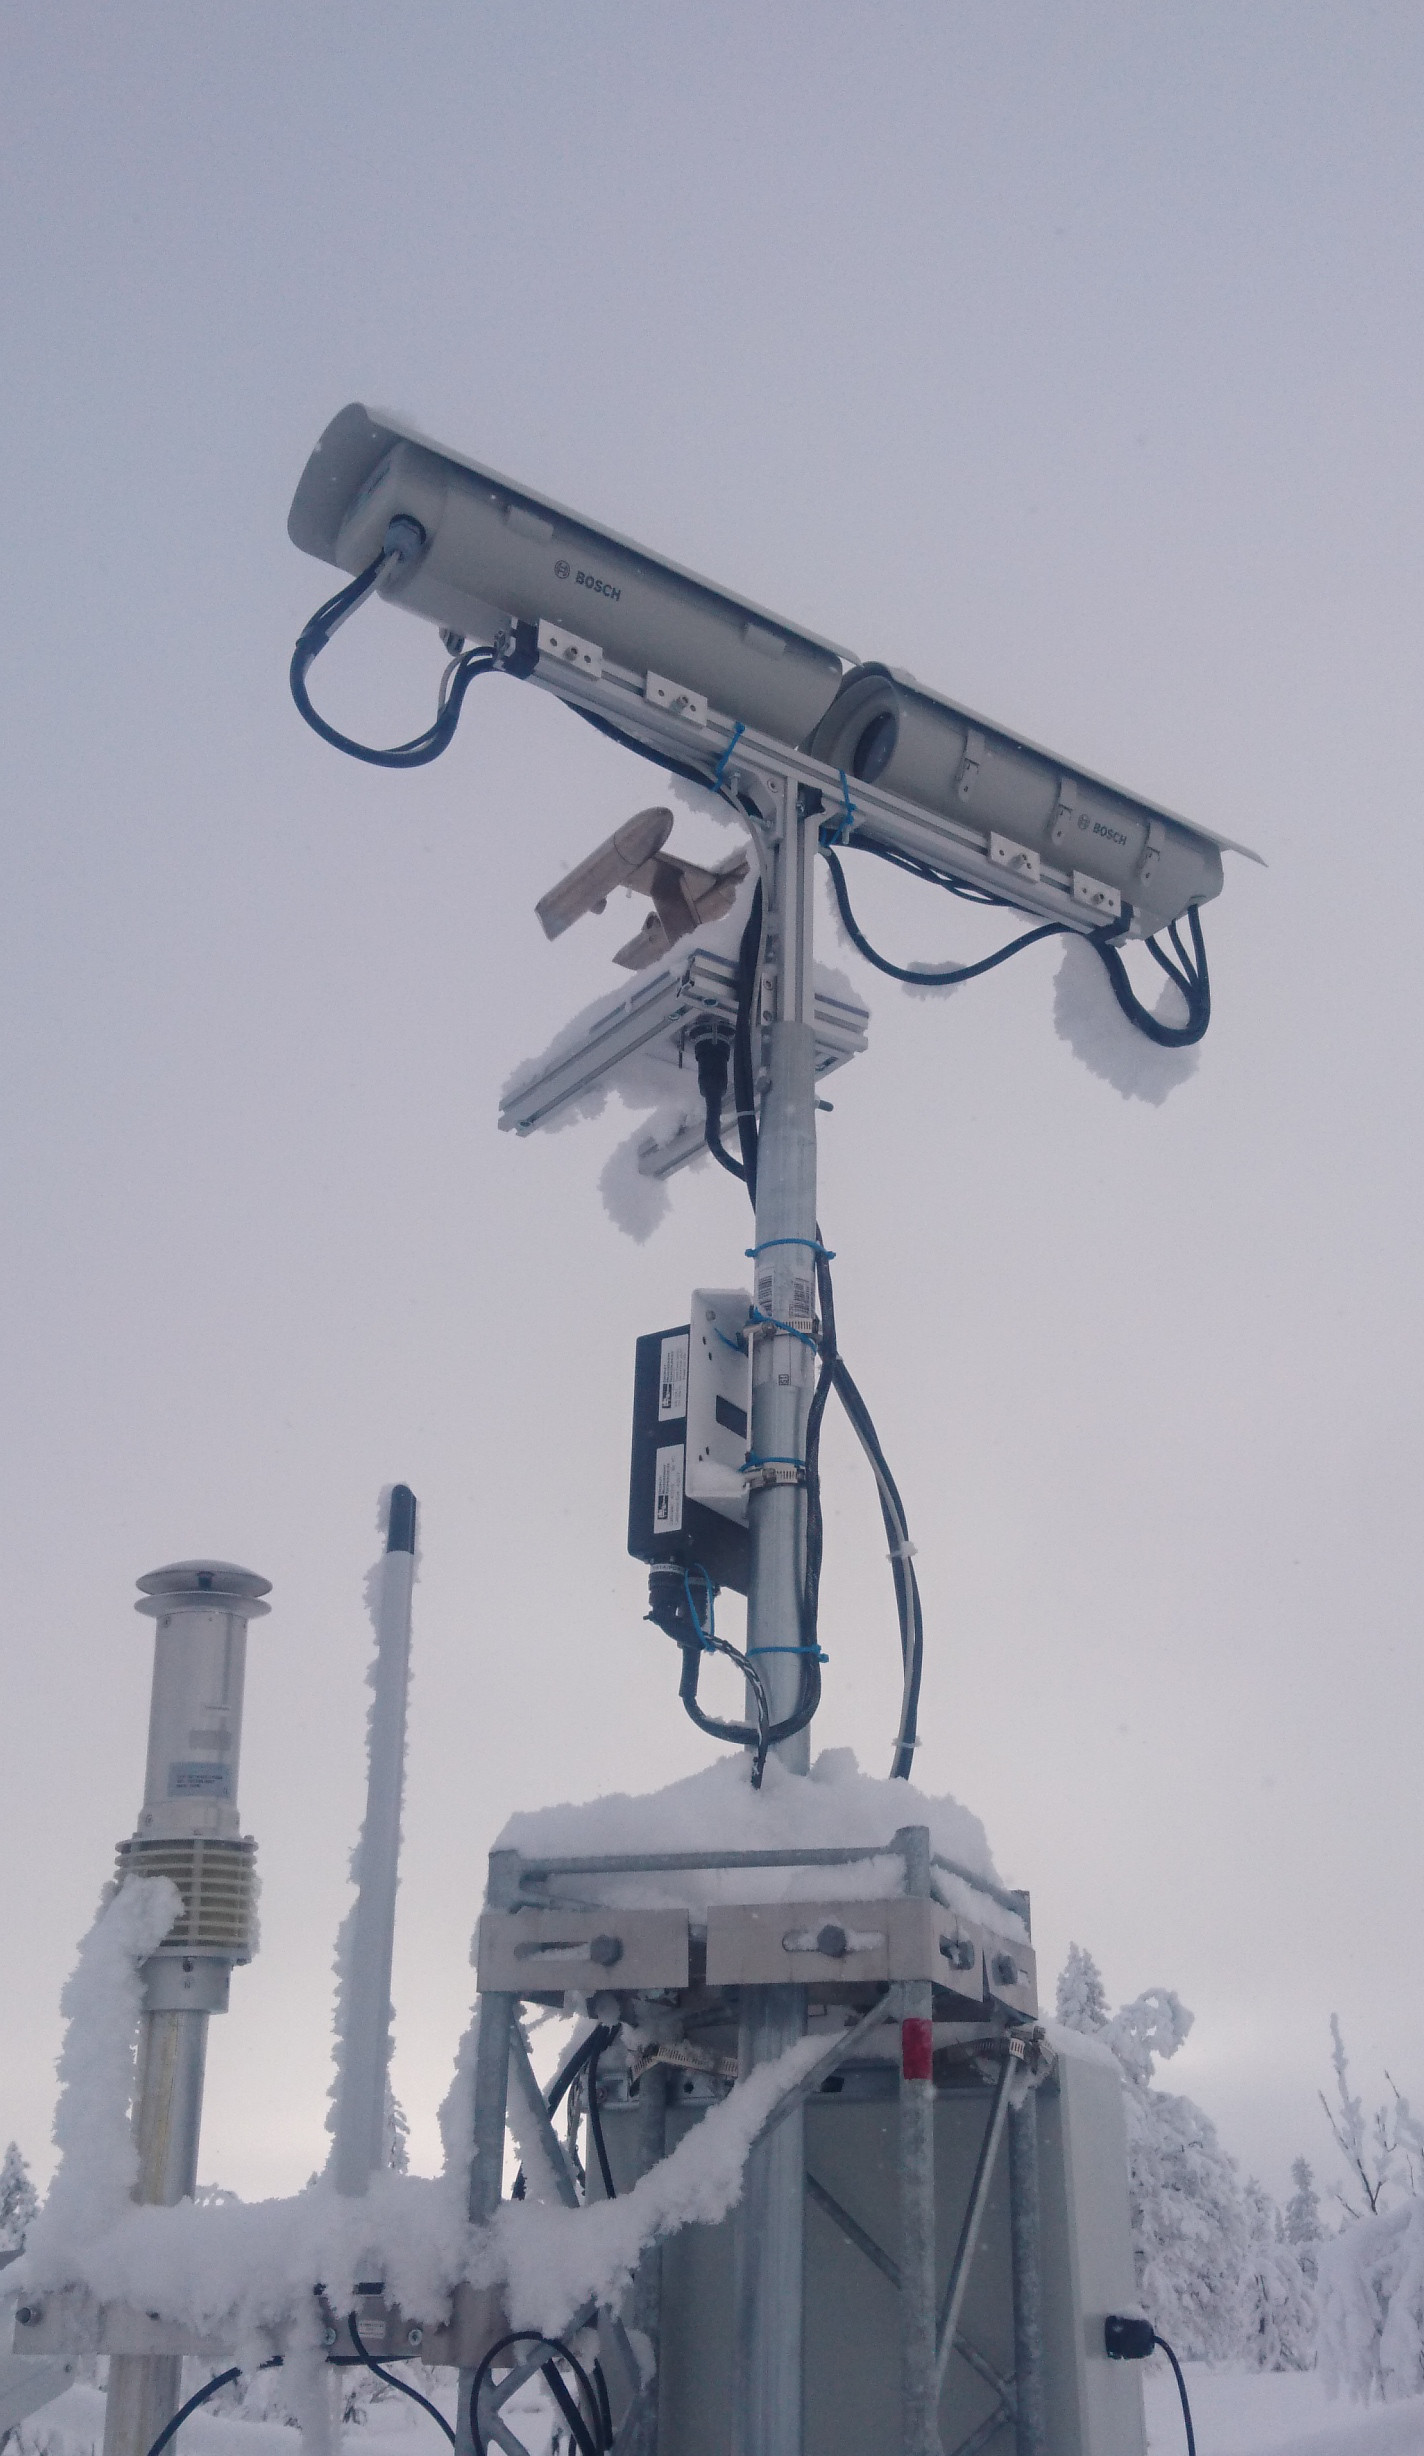
\includegraphics[width=0.75\linewidth]{figures/installation1}
\caption{Installation in Klövsjö.}
\label{fig:installation1}
\end{figure}

\begin{figure}[ht]
\centering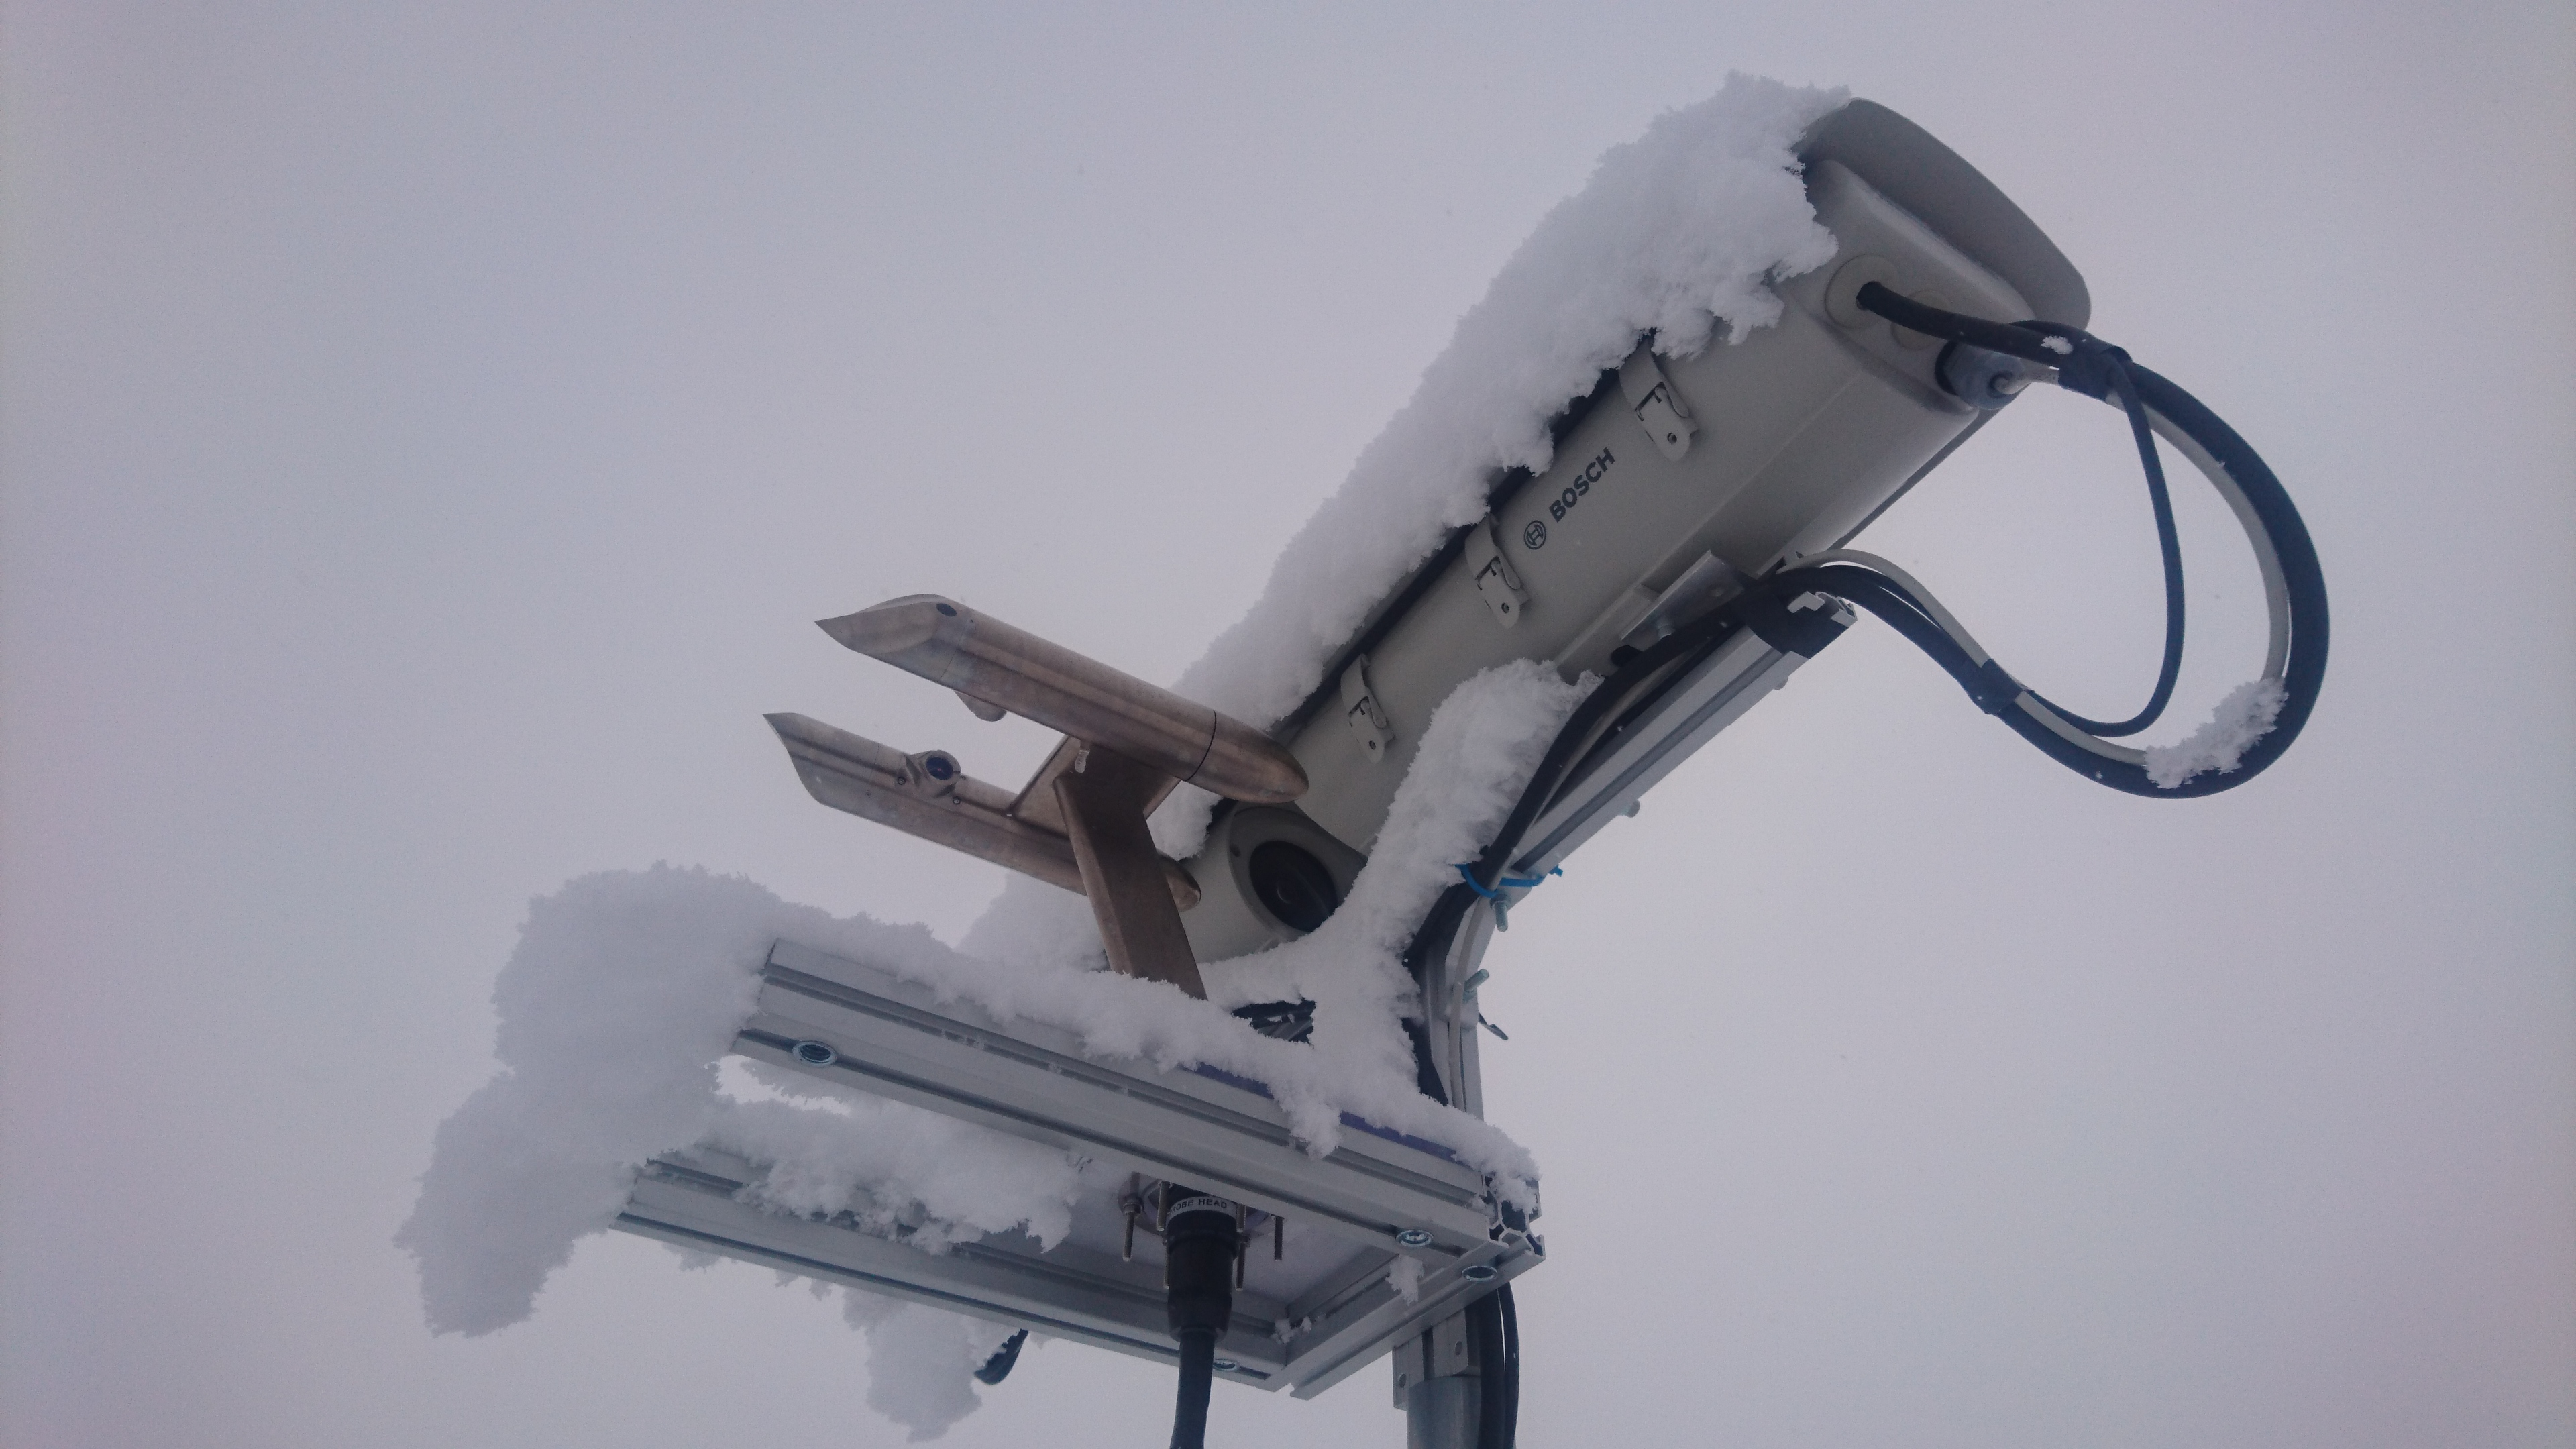
\includegraphics[width=0.75\linewidth]{figures/installation3}
\caption{Ice and snow on the front side of the installed instruments. The CDP is more efficient at preventing ice.}
\label{fig:installation3}
\end{figure}

\section{Numerical Weather Prediction}

For a second validation, we carry out weather simulations around the site using the \gls{harmonie}-\gls{arome} numerical weather prediction (\gls{nwp}) model. The model is described in Paper III.

\gls{smhi} agreed to run a special model domain locally with 500 meters horizontal resolution for a limited time. The operational forecasts are run at 2.5 km horizontal resolution, and they were used as initial conditions and lateral boundaries for the detailed simulations.

At \gls{smhi}, the \gls{harmonie}-\gls{arome} model is used for short range operational forecasting. It is run in cooperation with the Norwegian Meteorological Institute. The initial conditions and boundaries for the operational forecasts are provided by the \gls{ecmwf} global model.

\begin{figure}%[h]
\centering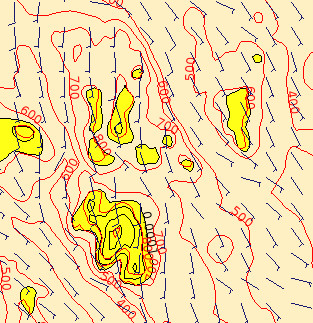
\includegraphics[width=0.6\linewidth]{figures/Images/Klovsjo_smhi160923_small}
\caption{Graphical presentation of data from the HARMONIE-AROME NWP covering Klövsjö and the surrounding mountains at a specific point in time using 500 m resolution. Yellow areas are where the model predicts an LWC more than 0.1 $\mathrm{g \cdot kg^{-1}}$. (Grams of water per kg air.) Simulation and figure by SMHI.}
\end{figure}



% this is shows the paper size and measures
%\begin{figure}
%    \oddpagelayouttrue
%    \twocolumnlayoutfalse
%    \stockdiagram
%    \caption{Right-hand page major layout parameters for
%        the \file{memoir} class} \label{fig:mempplt}
%\end{figure}
%\stockvalues
%
% !TeX root = ../main.tex
% !TeX spelling = en_GB
% !TeX program = pdflatex

\chapter{Results}
\label{chap:results}

The contents of this chapter are also found in Paper III. This result shown here can be seen as the answers to research question RQ4, and partly RQ5 from \Cref{chap:intro}.

\section{Measurement of Polymer Microspheres}

Four NIST calibrated distributions of microspheres, approximately 5, 10, 20 and 50 µm in diameter were used, resulting in four different measured size distributions. All images were saved and visually inspected, resulting in some measurement outliers due to clogging of smaller particles or contamination of small particles among larger. The outliers that were identified as not of the real distribution are not included in the result shown. Histograms of the measurement can be found in Figure \ref{fig:Histograms}. A summary of the result is shown in Table \ref{tab:poly_meas}.

\begin{figure}[ht]
\centering
\begin{subfigure}{.5\textwidth}
  \centering
  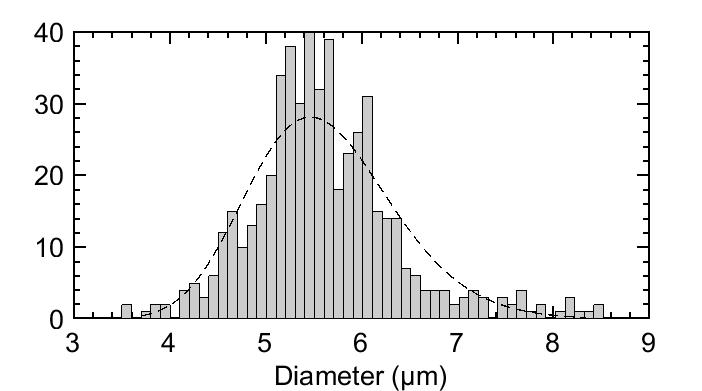
\includegraphics[width=1\linewidth]{figures/Images/Measurement1_5um}
  \subcaption{Distribution I.}
  \label{fig:Meas1_5um}
\end{subfigure}
\begin{subfigure}{.49\textwidth}
  \centering
  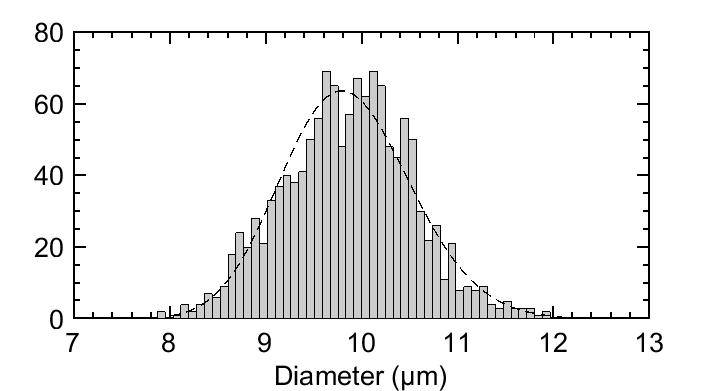
\includegraphics[width=1\linewidth]{figures/Images/Measurement1_10um}
  \subcaption{Distribution II.}
  \label{fig:Meas1_10um}
\end{subfigure}
\begin{subfigure}{.5\textwidth}
  \centering
  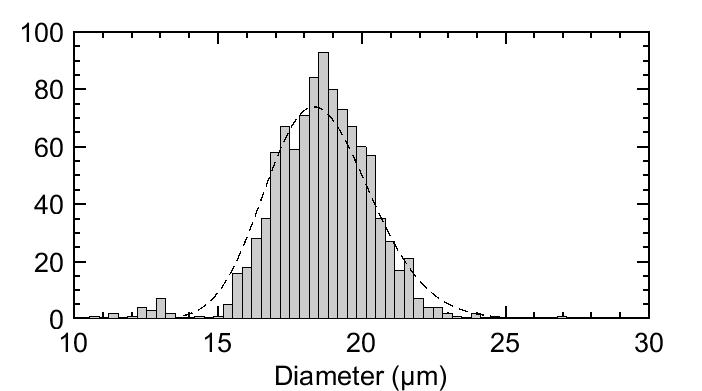
\includegraphics[width=1\linewidth]{figures/Images/Measurement1_20um}
  \subcaption{Distribution III.}
  \label{fig:Meas1_20um}
\end{subfigure}
\begin{subfigure}{.49\textwidth}
  \centering
  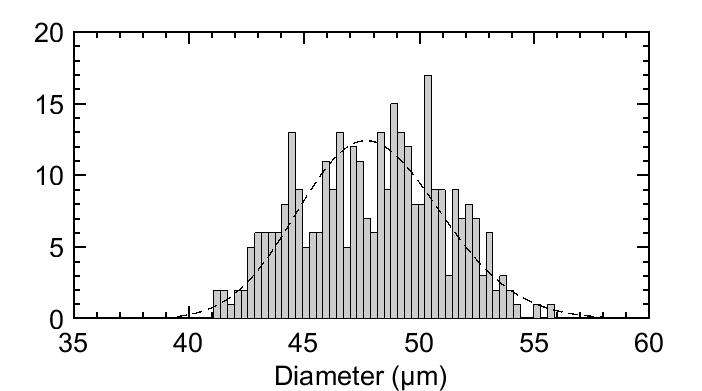
\includegraphics[width=1\linewidth]{figures/Images/Measurement1_50um}
  \subcaption{Distribution IV.}
  \label{fig:Meas1_50um}
\end{subfigure}
\caption{Histograms of the four measured distributions. The dashed line is a fitted  lognormal of the weighted distribution.}
\label{fig:Histograms}
\end{figure}

\begin{table}[ht]
\centering
\begin{tabular}{p{0.32\linewidth} p{0.14\linewidth} p{0.14\linewidth} p{0.14\linewidth} p{0.14\linewidth}}
\hline
\textbf{Distribution} & \textbf{I} & \textbf{II} & \textbf{III} & \textbf{IV}\\
\hline
Stated mean diam. & 5.3\newline \hspace{1em} ($\pm$ 0.3) & 10.3\newline \hspace{1em} ($\pm$ 0.4) & 19.1\newline \hspace{1em} ($\pm$ 0.7) & 49.4\newline \hspace{1em} ($\pm$ 1.6) \\
Measured mean diam. & 5.6 & 9.9 & 18.6 & 48.0 \\
\hline
Stated std. dev. & 0.5 & 0.9 & 1.7 & 3.5 \\
Measured std. dev. & 0.77 & 0.67 & 1.7 & 3.1 \\
\hline
\end{tabular}
\caption{Summary of the result from the measurement of NIST certified microspheres. All values are in µm.}
\label{tab:poly_meas}
\end{table}

\section{Comparison of DII and CDP Data}

Figure \ref{fig:0228-0301_MVD_DIIvsCDP} shows the MVD measured by the CDP compared with the DII. The least squares method applied on the data set results in a slope of 0.77 and a very small offset of -0.3 µm. Ideally, if both instruments were measuring the true diameter, the slope here would be equal to 1. A straight line with a slope that is not equal to 1 means that there is a systematic difference between the CDP and the DII in the size measurement.

\begin{figure}[ht]
\centering
\begin{subfigure}{.85\textwidth}
  \centering
  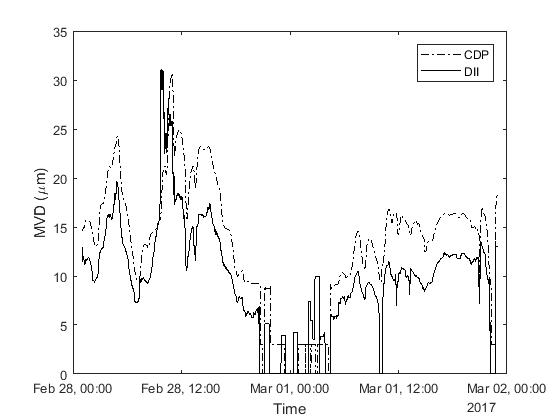
\includegraphics[width=1\linewidth]{figures/0228-0301/30min_mvd_CDP_DII_170228-170301_19212_0LpartDII_214646_0LpartCDP}
  \subcaption{MVD vs. time}
  \label{fig:0228-0301_MVDvstime}
\end{subfigure}%

\begin{subfigure}{.85\textwidth}
  \centering
  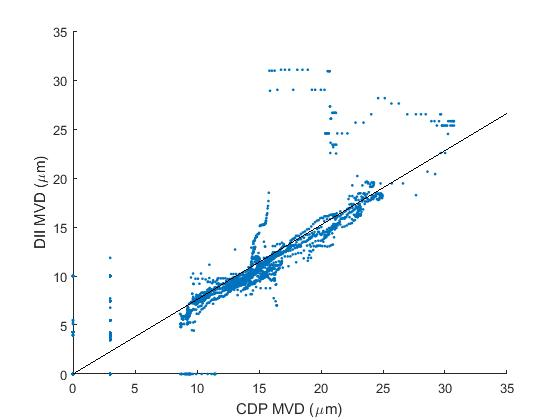
\includegraphics[width=1\linewidth]{figures/0228-0301/Mvdquote_DII-CDP_17022801-17030123_2760min_leastsquare0_7682}
  \subcaption{MVD measured by DII versus CDP}
  \label{fig:0228-0301_MVD_DIIvsCDP}
\end{subfigure}
\caption{MVD minute values measured by the DII and the CDP for 46 hours on 28-02-2017--01-03-2017.}
\label{fig:0228-0301_mvd}
\end{figure}

We compare the instruments by studying the data from 28 February to 1 March. See Figure \ref{fig:0228-0301_lwc} and \ref{fig:0228-0301_mvd}. Figure \ref{fig:0228-0301_LWC_DIIvsCDP} shows the LWC measured by the CDP compared with LWC measured by the DII. Using the least square method on the whole data set gives an average quote of 0.27. The quote is drawn in the plot as a straight line from the origin. Here too, the ideal case is a straight line with the slope equal to 1. The difference is discussed in \Cref{sec:systemdiff}.

\begin{figure}[ht]
\centering
\begin{subfigure}{.85\textwidth}
  \centering
  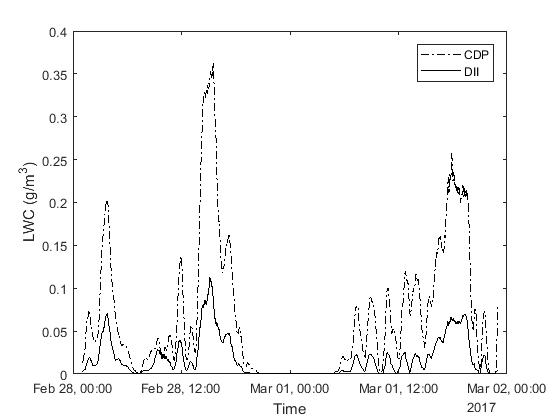
\includegraphics[width=1\linewidth]{figures/0228-0301/30min_lwc_CDP_DII_170228-170301_19212_0LpartDII_214646_0LpartCDP}
  \subcaption{LWC as a function of time}
  \label{fig:0228-0301_LWCvstime}
\end{subfigure}%

\begin{subfigure}{.85\textwidth}
  \centering
  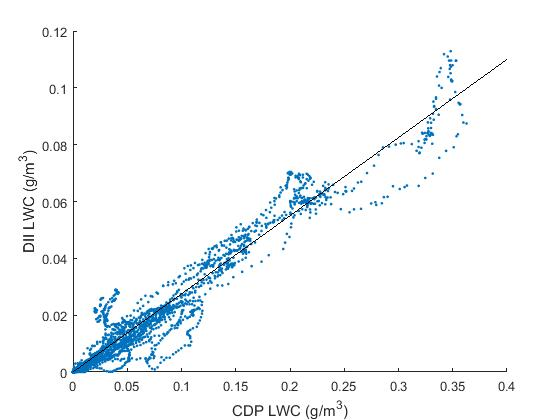
\includegraphics[width=1\linewidth]{figures/0228-0301/Lwcquote_DII-CDP_17022801-17030123_2760min_leastsquare0_2742}
  \subcaption{LWC measured by DII versus CDP}
  \label{fig:0228-0301_LWC_DIIvsCDP}
\end{subfigure}
\caption{LWC measured by the DII and the CDP for 46 hours on 28-02-2017--01-03-2017.}
\label{fig:0228-0301_lwc}
\end{figure}

\clearpage
The quote between the LWC values of the two instruments is plotted together with the wind speed in Figure \ref{fig:0228-0301_WSvslwcquote}. The least square average is plotted as a horizontal line at 3.65 (CDP LWC/DII LWC). The logarithmic scale is cropped with 238 quote values above 100 and 121 values below 0.1 out of a total of 2760.

\begin{figure}[ht]
  \centering
  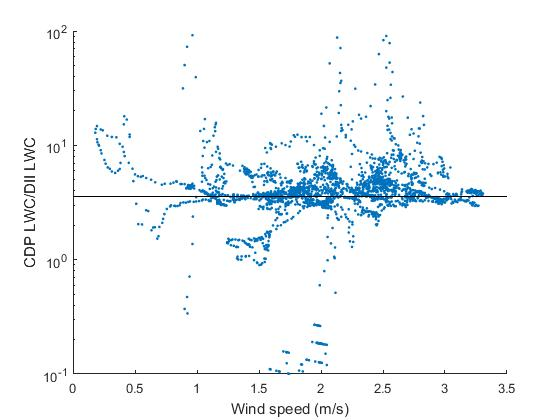
\includegraphics[width=0.85\linewidth]{figures/0228-0301/Relation_between_lwcquote_and_wind_speed_17022801-17030123}
\caption{Relation between the wind speed and the quote between the LWC measured by the CDP and the DII. The vertical scale is cropped at 1 and 100. 238 values are above 100 and 121 below 1 out of a total of 2760.}
\label{fig:0228-0301_WSvslwcquote}
\end{figure}

\clearpage
\section{Comparison of Measured and Modeled Data}

Figure \ref{fig:161211_mvd_lwc} shows the LWC and the MVD from the two instruments compared with the data from the HARMONIE-AROME model at 500 m resolution. The fog lasted for about 19 hours on 12-11-2016. The difference between the two instruments follows the same systematic pattern during this specific measurement, as in all the other observations. The HARMONIE-AROME model data of the LWC follows the general data of the LWC but fails to detect the large increase in LWC between 05:00 and 12:00. The predicted MVD of the model is closer to the actual values of the DII than the CDP.

\begin{figure}[ht]
\centering
\begin{subfigure}[t]{.85\textwidth}
  \centering
  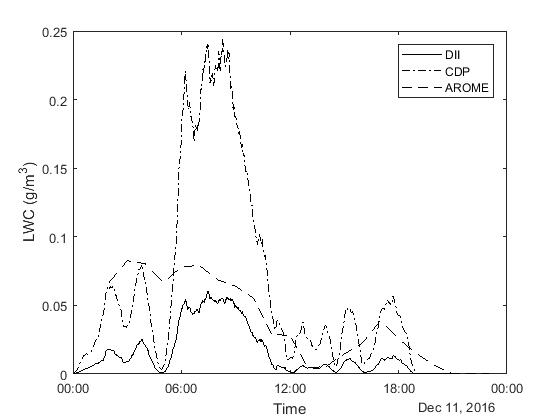
\includegraphics[width=1\linewidth]{figures/161211/30min_lwc_CDP_DII_SMHI_161211_adjusted}
  \subcaption{LWC vs. time}
  \label{fig:161211_LWCvstime}
\end{subfigure}%

\begin{subfigure}[t]{.85\textwidth}
  \centering
  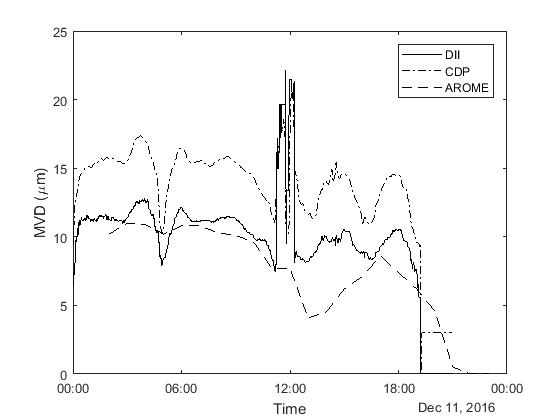
\includegraphics[width=1\linewidth]{figures/161211/30min_mvd_CDP_DII_SMHI_161211_adjusted}
  \subcaption{MVD vs. time}
  \label{fig:161211_MVDvstime}
\end{subfigure}
\caption{LWC and MVD measured by the DII and the CDP 11-12-2016. HARMONIE-AROME model data using 500 meter resolution. }
\label{fig:161211_mvd_lwc}
\end{figure}

\clearpage
Figure \ref{fig:0203-0206_lwc_mvd} shows the result from measurement 03-02-2017--06-02-2017. Unfortunately, no data from the CDP was saved at this point, due to a full memory. The double spike in the MVD diagram \ref{fig:0203-0206_MVDvstime} at 04:17 and 04:41 on 05-02-2017 is mainly caused by two droplets, 51 and 74 µm (see Figure \ref{fig:170505_0441_droplet}) in combination with a number of large droplets between 30 and 40 µm in diameter.

\begin{figure}[ht]
\centering
\begin{subfigure}[t]{.85\textwidth}
  \centering
  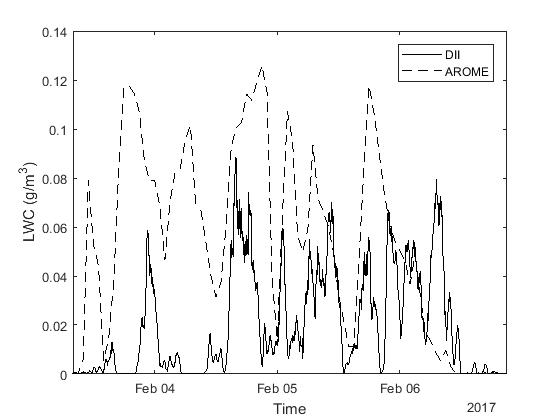
\includegraphics[width=1\linewidth]{figures/0203-0206/30min_lwc_foggy_smhi_170203-170206_86h}
  \subcaption{LWC vs. time.}
  \label{fig:0203-0206_LWCvstime}
\end{subfigure}%

\begin{subfigure}[t]{.85\textwidth}
  \centering
  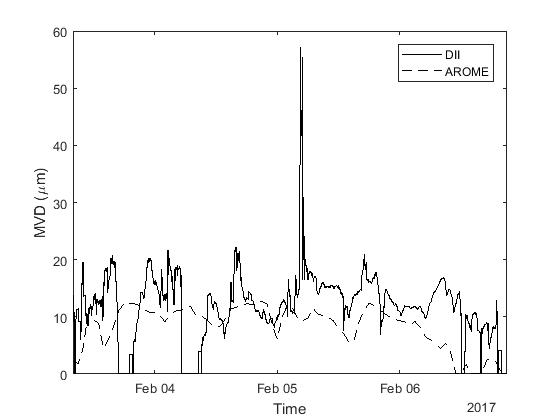
\includegraphics[width=1\linewidth]{figures/0203-0206/30min_mvd_foggy_smhi_170203-170206_86h}
  \subcaption{MVD vs. time.}
  \label{fig:0203-0206_MVDvstime}
\end{subfigure}
\caption{LWC and MVD measured 03-02-2017--06-02-2017 by the DII. HARMONIE-AROME model data using 2.5 km resolution, stored every 60 minutes.}
\label{fig:0203-0206_lwc_mvd}
\end{figure}

\begin{figure}[ht]
\centering
\begin{subfigure}[t]{.8\textwidth}
  \centering
  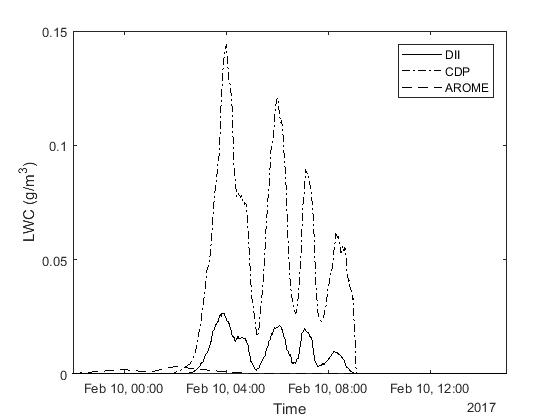
\includegraphics[width=1\linewidth]{figures/170210/30min_lwc_CDP_DII_SMHI_170210_2263part}
  \subcaption{LWC vs. time.}
  \label{fig:170210_LWCvstime}
\end{subfigure}%

\begin{subfigure}[t]{.8\textwidth}
  \centering
  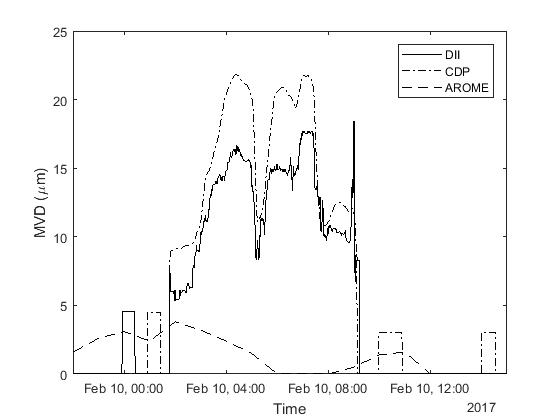
\includegraphics[width=1\linewidth]{figures/170210/30min_mvd_CDP_DII_SMHI_170210_2263part}
  \subcaption{MVD vs. time.}
  \label{fig:170210_MVDvstime}
\end{subfigure}
\caption{LWC and MVD measured by the DII and the CDP 10-02-2017. HARMONIE-AROME model data using 2.5 km resolution, stored every 60 minutes.}
\label{fig:170210_lwc_mvd}
\end{figure}


%
% !TeX root = ../main.tex
% !TeX spelling = en_GB
% !TeX program = pdflatex

\chapter{Discussion}
\label{chap:discussion}

\section{Starting Studies}
\label{sec:discussionstarting}

\subsection{Infrared and Visible Light}

The amound of absorbed light in a small water droplet is close to negligible compared to the scattered light. In a large ensemble of droplets, such as a cloud, the total absorption will still be significant, especially for wavelengths in the near and far infrared. Since it was possile, we made a quick comparison of illumination using blue light (ca 450nm) and near infrared (ca 850nm). The blue light gave the sharpest image, probably due to the sensor's slightly higher sensitivity for blue light. But also possibly due to the higher theoretical resolving power as described by Rayleigh's criterion. See Paper I.

\subsection{Laser Light}
\label{sec:discussionlaser}

Lasers are used in numerous optical instruments for droplet measurement, and there is good reason to. Prices for high power semiconductor lasers have become very attractive. With a laser it is possible to achieve a short light pulse with a high energy. The coherency causes strong diffraction patterns, something that is used when reconstructing images in holographic imaging instruments This makes it possible to achieve a larger measuring range than what is possible in conventional imaging, as mentioned in section \ref{sec:relwork}. Sizing of particles can still be difficult, in addition to more calculation intensive. 
 
Laser illumination was tried used using two wavelengths, 450 and 850 nm and placed in different positions. \Cref{fig:laser} shows an example image with a 450 nm laser placed about 135 degrees from the optical center. Direct size and concentration measurement is difficult for at least following reasons: 
\begin{enumerate}
\item The measurement volume is difficult to define because the laser light intensity is spatially inhomogenous.
\item The light intensity in the measurement point is difficult to control. Overexposure makes the glare appear larger.
\item Interference patterns from particles outside the measurement volume is disturbing the measurement.
\end{enumerate}

\begin{figure}%[ht]
\centering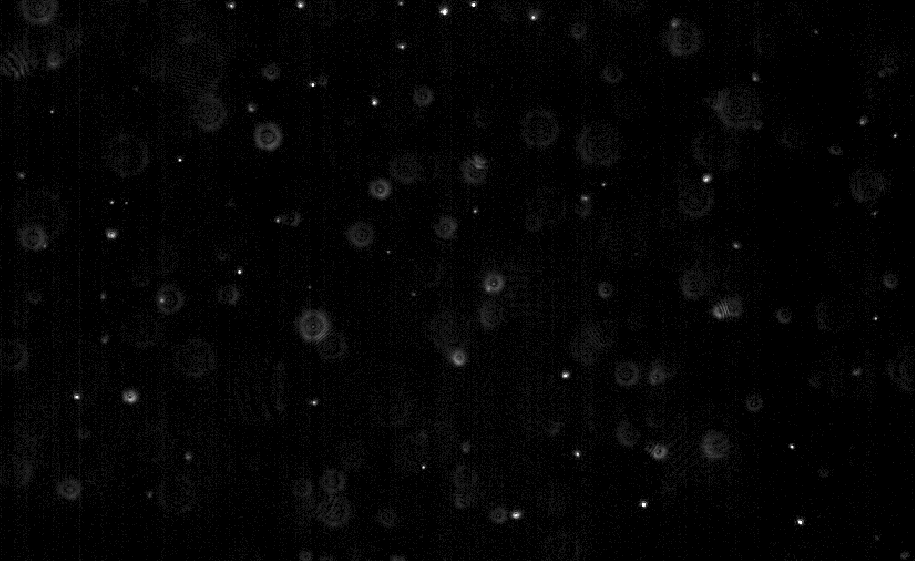
\includegraphics[width=0.6\linewidth]{figures/450nm45deg}
\caption{Reflections and interference patterns 450nm laser light. The light source is placed at a position about 135 degrees from the optical center.}
\label{fig:laser}
\end{figure}

For conventional imaging of small particles the coherence mainly causes problems. Although it is possbile to make the laser incoherent e.g. by using diffusers or optical fibres, it is just one of the things that makes the complete system slightly more complex.

\subsection{Exposure Energy Measurement}
\label{sec:expmeasurement}

The measurement is also described in Paper I. The result is shown in \Cref{fig:expenergy}. The energy was measured by using a thermal power sensor, the area of view and the time that is required for a full exposure. 34 nJ is required for the area in view (7.8 $mm^2$) for the lowest gain setting, which results in the highest SNR and about 20 nJ for the used setting.

\begin{figure}[ht]
\centering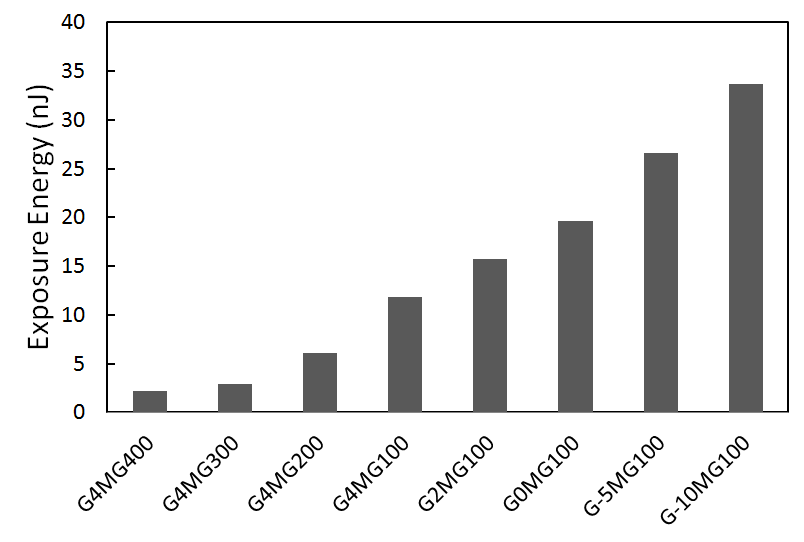
\includegraphics[width=0.75\linewidth]{figures/Energy_per_gain_level2}
\caption{Light energy ($nJ$) for exposure in each of the eight gain levels used. The energy was tuned manually up to a level of high exposure, but not saturating any point in the image.}
\label{fig:expenergy}
\end{figure}

\subsection{Ambient Light}

The shortest possible exposure time according to the camera specification is 0.038 ms, slightly depending on other camera settings. For each measurement 152 images were captured, with an increasing exposure time from ca 0.04 to 1.99 ms. A delay of 1 second was set between each image. \Cref{fig:ambientlight} shows the mean pixel value and the standard deviation of the value for one of the measurements at 22000 lux ambient light.

\begin{figure}%[ht]
\centering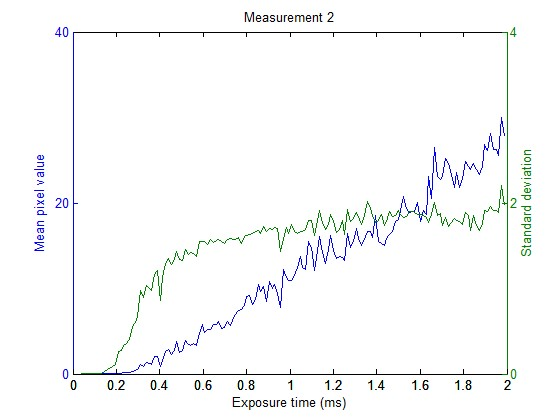
\includegraphics[width=0.6\linewidth]{figures/Amblight22000lux}
\caption{Mean pixel value and standard deviation of ambient for a light measurement at 22000 lux.}
\label{fig:ambientlight}
\end{figure}

Using this setup it was found that an exposure time of at least one second is needed to give a signal that is comparable to the noise level under normal exposure. At the same time, in order to image small droplets, the exposure time needs to be less than one μs. Therefore we concluded that the ambient daylight would likely have no effect on the measurement.

\section{Image Noise and SNR}

We observed a correlation between the \gls{snr} and the corresponding measuring range, resulting in an increased sampling volume for higher \gls{snr} \cite{ryd2015}(Paper I). This relation has not yet been implemented in the LWC calculation for the prototype instrument.

The \gls{snr} for a ten micrometer dot image was calculated using seven gain level settings of the image sensor. For each gain level, the illumination time was adjusted so that the level of exposure was the same. This measurement was done using both the 455 and the 850 nm illumination. The result can be seen in \Cref{fig:noisegain}. Lower gain levels require longer light pulses, but results in higher \gls{snr}. It can also be seen that the \gls{snr} for 455 nm is systematically higher than for 850 nm. 

\begin{figure}%[ht]
\centering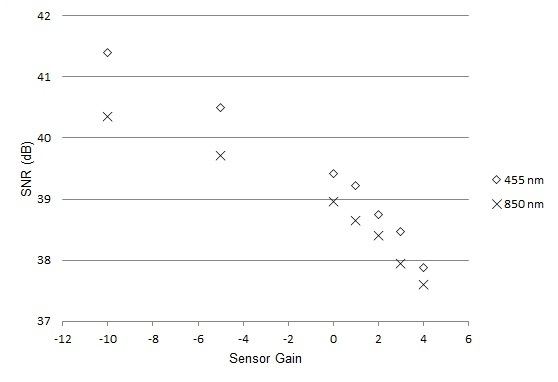
\includegraphics[width=0.6\linewidth]{figures/NoiseGain}
\caption{SNR for a ten micrometer dot image using two wavelengths and seven gain level settings. Shorter wavelength and lower gain gives less noise.}
\label{fig:noisegain}
\end{figure}

The design using a weakly collimated LED that illuminates an area slightly larger than the field of view makes the system quite insensitive to misalignment of the camera and the light source. Temporal or permanent changes in light intensity caused by a minor misalignment can be automatically compensated for by continuous measurement of the total exposure level. If the level of exposure is increasing or decreasing, the length of the light pulse is changed correspondingly. The light intensity can also be affected by dirt on the front glass of the housings. 

Spatial dissimilarities in the light intensity that are not caused by noise we can compensate for by calculating the local average intensity of the background around each measured droplet. The size of a droplet is then based on the intensity dip caused by the shadow compared with its local background.

\section{Image Pre-processing}

To increase the number of processed images a pre-process is done using a variable threshold as described in section \ref{imgsegment}. The processing speed could be increased even more limiting the edge detection algorithm to the region or regions around the discovered differences.

\section{Aerodynamics}

Many existing instruments suffer from errors caused by the instrument itself during sampling, e.g. when droplets get stuck on the inlet or shatters into smaller droplets. The DII is not as small and aerodynamically shaped as the \gls{cdp}, therefore a difference between the instruments would be expected depending on the air speed. However, a comparison between the measured values of LWC showed no connection between the wind speed and the difference in the measured LWC. The wind speed during the comparison was only 1-4 $\mathrm{m \cdot s^{-1}}$ which probably explain why the less aerodynamic shape of the DII compared with the \gls{cdp} has no noticeable effect. This could change dramatically when measuring at higher wind speeds.

\section{Difficulties in the Polymer Microspheres Measurement}

To verifiy the sizing algorithm, a measurement using polymer microspheres of four known calibrated size distributions was done. To simulate real conditions as much as possible the microspheres were applied using the same dispenser used for the calibration of the \gls{cdp}. The smallest microspheres had a tendency of clogging leading sometimes to a measurement of a clog as a single particle. Therefore all images were visually checked for false measurements. The outliers caused by false measurements were removed.

\subsection{Clogging}

Small microspheres are forming larger clogs that are measured as single microspheres. The reason may be static electricity or humidity. As can be seen in the five micrometer measurement, the result of some clogs becomes outliers in the expected distribution. This needs to be considered when solid microspheres are used as reference objects. Colliding liquid water droplets would of course coalesce into larger droplets, thereby changing the diameter.

The equipment and the dispenser was thoroughly cleaned using compressed air between each measurement. Still there may be microspheres or other contamination left, changing the distribution slightly.

Measured mean and standard deviation of all distributions were found to be within the stated calibrated values. This can be seen as a confirmation that the instrument calibrated only by the micrometer dot scale is measuring the microsphere samples correctly.

\subsection{Roundness}

A perfectly circular disc measured using an infinite resolution would have an expected roundness value equal to one. In practice, this is not possible to achieve in a digital image. But the contour is only used as detection criteria. Instead, the diameter is calculated using the negative shadow intensity. Therefore the contour roundness itself should not have very large impact on the accuracy.

The roundness criteria defined in chapter \ref{met:roundness}. The roundness (\ref{eq:5}) limit set at 0.85 in this measurement seems to work fine. It excludes most irregular objects, like clogs in the five micrometer measurement. When measuring fogs in cold climates, the water droplets will be mixed with ice crystals. While larger crystals will mostly be sorted out by the roundness criteria, crystals smaller than ten micrometer may be difficult, and five micrometer crystals more or less impossible to distinguish from liquid water droplets unless very different in shape.

\begin{figure}[ht]
\centering
\begin{subfigure}[t]{.5\textwidth}
  \centering
  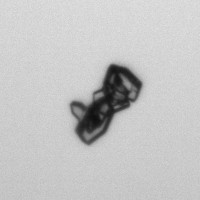
\includegraphics[width=1\linewidth]{figures/litenis1}
  \subcaption{Ice particle.}
  \label{fig:litenis}
\end{subfigure}%
\begin{subfigure}[t]{.5\textwidth}
  \centering
  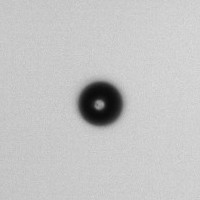
\includegraphics[width=1\linewidth]{figures/litendroppe1}
  \subcaption{Droplet.}
  \label{fig:litendroppe}
\end{subfigure}
\caption{Difference between an ice particle and a water droplet that is 62 µm in diameter. Larger ice and snow particles tend to be more complex in shape. Ice particles smaller than 10 µm in diameter may be difficult to distinguish from water droplets.}
\label{fig:icevsdrop}
\end{figure}

\subsection{Calibration Validation}

The calibration functions derived from the measurement of known sized dots is an approximation and an interpolation. It is based on the assumption that light scatters similarly on the edge independently of the size of the object. This is not quite true, especially for smaller particles \cite{bohr2008}. For particles around ten micrometer or less in diameter we would expect different intensities forming a diffraction pattern close to the edge. The pattern would be stronger the more coherent the illumination. In this system, using LED illumination, the coherence length is short enough that no patterns are visible. Still changes to the edge for the smallest diameters can still not be altogether ruled out.

The experiment using calibrated spheres confirms that the measurement of droplet diameters is accurate. It is however not a confirmation of the measurement volume \cite{ryd2016} since we do not know the concentration of the microspheres. This means that we cannot yet confirm an accurate measurement of the LWC. To do that, an independent verification of the measurement volume is needed.


\section{LED Illumination}

Using a high power LED instead of laser reduces the interference effects used in e.g. holography \cite{henn2013}, but since it is a monochromatic source, interference may not be completely ruled out. The coherence length for the blue LED is calculated in Paper I.

One would expect diffraction patterns depending on the spectral bandwith of the light source. The narrower the bandwidth, the stronger the diffraction. A spectrum analysis of the \gls{led} showed that the coherence length of the blue \gls{led} is about 6.8 μm. Therefore the spectrum was measured using a spectrum analyzer. The result can be seen in \Cref{fig:ledspectrum}.

\begin{figure}%[ht]
\centering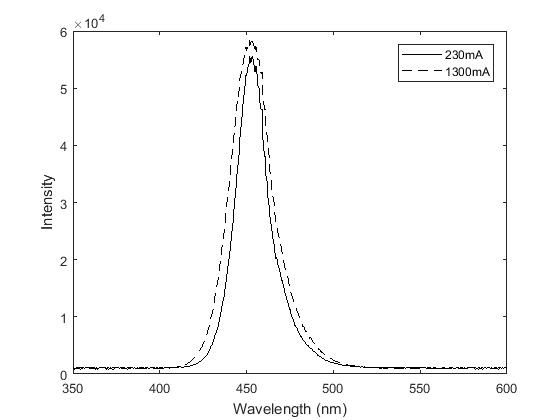
\includegraphics[width=0.6\linewidth]{figures/spektralanalys_mightex455nm}
\caption{Spectrum of the Mightex 455nm \gls{led} using two different driving currents. The band width is slightly wider for the higher current.}
\label{fig:ledspectrum}
\end{figure}

LEDs can sometimes be used with currents far above the specifications, as long as the pulse length is short and the duty cycle is low enough to permit the heat generated to be transported away between the pulses. Using the LED above specifications may though affect the efficiency and aging of the LED. LED emittance also depends on the temperature. Depending on the capacitance of the diode, the rise time may limit the current, although there exist some techniques to shorten the LED pulses \cite{tanaka2011,vele2007}.

The LED used was fully functional after four months of measurements using a current in the short flashes that was 12 times higher than the maximum continous current specified by the manufacturer. At 12 ampere driving current, the flash duration could be lowered to approximately 250 ns, still using the normal settings of amplification in the camera. The LED was not tested in higher currents, but it seems possible that it could work. A question is how high current the LED can handle and how the lifetime is affected by higher driving currents.

\section{Statistics}

A value of both MVD and LWC can be derived from a series of images and since the number of measured droplets will depend on the concentration, the accuracy and precision will depend on the number of samples from the total population of droplets. 

In Paper I we made an estimation of the precision a possible instrument could have using the most ideal scenario, where the ''distribution'' was simulated using a single dot of a known size, measured multiple times. This can be seen as a measure of the highest possible precision, defined by the physical limitations of the system components. The coefficient of variation for the LWC was estimated to 1.6 percent for droplets 25 µm in diameter, and 2.4 percent for droplets 10 µm in diameter. In practice it is difficult to compare this with the measured LWC from a real  distribution of droplets. To know the exact LWC, and measure the same content is practically impossible. 

In Paper III, a comparison is made by measuring polymer microspheres in distributions calibrated by NIST. As can be seen in \Cref{tab:poly_meas}, the difference between the measured mean diameter and the stated mean diameter is small. This proves that the size measurement is accurate. It was not possible to estimate the concentration of the measured microspheres with the method we used. Possibly a known concentration could be produced in a water dispersion, but then the optical ambient conditions would also be different.


\section{Droplets and Size Distributions}

Droplets that are very close are likely to coalesce, thereby decreasing the number concentration at a rate that appears to increase for larger droplets and more complex droplet size distributions \cite{borda2011}. 

Due to the small depth of the measurement volume, i.e. the measuring range compared with the field of view, the likelihood of finding two droplets very close in the image is very low due to the low number concentration of droplets we are measuring. A solution is to make a measurement of the droplet’s circularity and add this as selection criteria for the measurement. This solution also works as a filter for ice or snow particles. 

The drop size distribution of cloud droplets 3-50 µm in diameter have usually been considered to follow a lognormal or gamma curve \cite{miles2000,lee2010,sein1998}. This also applies to rain \cite{ulb1983}. However, more recent measurements of drop size distributions show that the distribution greatly varies \cite{james2001,shaw2002,peters2005,cob2011}. Consequently, the results will depend on the measurement method and the sampling volume.

\subsection{Sampling Speed and Volume}

Since the DII has no external trigger of the imaging, the sampling speed, i.e. the volume of air and droplets that is scanned per time unit, depends on the measuring volume of each image and the imaging speed. 

The sampling speed of the CDP is linearly dependent on the wind speed. The sample area also depends on the size of the measured droplets, but the factory calibration value is given for all sizes. The sampling speed of the DII depends primarily on the image frame rate and the measurement range for each droplet size. At a wind speed of 2 m/s, the sampling speed of the CDP is $\mathrm{4.1 \cdot 10^{-7} m^{3} \cdot s^{-1}}$. This is 39 times higher than the sampling speed of the DII for 20 µm particles. To achieve the same sampling speed, the frame rate of the DII would need to be almost 200 $s^{-1}$. 

Despite the relatively low sampling speed and the small sampling volume of the DII, it seems that by averaging the LWC and the MVD over a period of 30 minutes, enough precision is achieved to be able to compare the two instruments. Since the purpose of the DII is primarily to detect conditions for icing on wind turbines, and provide in-situ observational data for NWP models, the achieved sampling speed may even be good enough, at least for the latter. If the speed is good enough to decide when to switch on de-icing on the blades depends on how quickly the ice builds up, and what de-icing method is used. During icing, high LWC and high MVD are expected.

When comparing the 30 min moving average values for the period 28 February -- 1 March, shown in \Cref{fig:0228-0301_LWCvstime} and \Cref{fig:0228-0301_MVDvstime}, there is very good agreement between the curves, with the exception of 11.30-12.00 when at least ten droplets 25-35 um in diameters were measured by the DII, resulting in a significantly higher MVD and LWC measured by the DII than the CDP. The reason why the CDP did not measure any similarly sized particles on this particular occasion is not known. There is also a difference in the MVD when the LWC is very low resulting in a small number of measured droplets.

The sampling speed could be raised by e.g. changing the optical magnification but then at the cost of a lower optical resolving power. Different ideas to increase the sampling speed of the DII are discussed in Paper I and Paper II.

Another way of increasing the sampling speed is to increase the imaging speed. Cameras with a high imaging speed exist and the flash pulse is so short that it would still be a low duty cycle for the LED. The most limiting factor is problably the processing time. This can be solved by implementing parts of the image processing in hardware.

The speed requirement finally depends on the application. If the instrument is used for the verification of NWP models, the sampling speed of the prototype may be enough. If the instrument is supposed to be used for triggering de-icing, the sampling speed may need to be increased.

\subsection{Large Droplets}

The CDP does not measure particles larger than 50 µm. But if the distribution of droplets was following a lognormal, or gamma curve \cite{miles2000,lee2010} also for particles larger than 50 µm, enough large droplets should have been detected by the CDP to see an increase in the measured MVD. As demonstrated, this was not always the case. A possible explanation is that the larger cloud droplets do not follow the lognormal distribution when they are above a certain size. If this is true, the predicted MVD may be less useful for the description of a cloud aerosol distribution, as well as for conclusions about possible icing. In the case with supercooled large droplets, the LWC may be more important to measure than the MVD. But to fully understand this, a parallel measurement using an ice load instrument is required.

\Cref{fig:170505_0441_droplet} and Figure \Cref{fig:170505_1648_droplet} show supercooled large droplets measured during the fog on 05-02-2017.

\begin{figure}[ht]
  \centering
  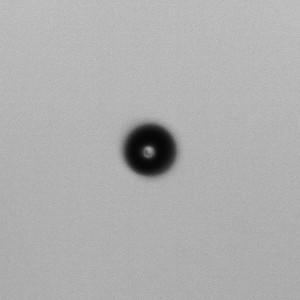
\includegraphics[width=0.4\linewidth]{figures/170205_0441_droplet_74um}
\caption{A 74 µm droplet detected at 04:41 on 05-02-2017.}
\label{fig:170505_0441_droplet}
\end{figure}
\begin{figure}[ht]
  \centering
  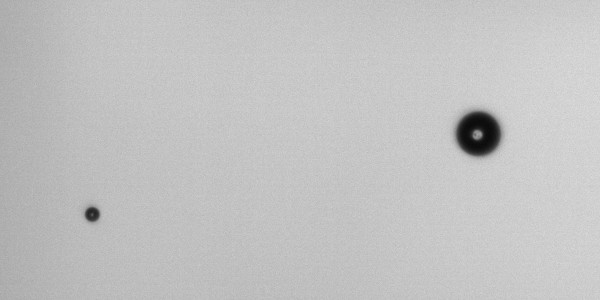
\includegraphics[width=0.8\linewidth]{figures/170205_1648_droplet_19and62um}
\caption{Two droplets, 19 and 62 µm in diameter detected in the same image at 16:48 on 05-02-2017.}
\label{fig:170505_1648_droplet}
\end{figure}


\section{Icing}

The risk of icing increases with increasing wind speed \cite{makk2000}.

During the field study there were several instances when the LWC and MVD was high enough to lead to icing. A study to further investigate the connection between these parameters and the ice load according to ISO 12494 \cite{makk2014} should be carried out. An ice monitoring device, like the Combitech IceMonitor \cite{cost727,thors2015} can be used for this. This should preferably be done in combination with a third independent LWC and MVD measurement, e.g. by using rotating cylinders \cite{makk1992,knez2005}. A heated hygrometer measuring the true water content (\gls{twc}) can be used as an alternative verification of the LWC measurement when all the atmospheric water is in liquid form \cite{spie2012}.







%
\chapter{Summary of the Thesis}
\label{chap:summary}

The thesis describes the work resulting in three scientific papers.

\section{General Conclusions}

Shadowgraph imaging can be used for comparison and validation of NWP models. The technique can also be used for size reference measurement of instruments based on other techniques. The accuracy of the particle size measurement is high. 

The accuracy of the concentration measurement is questioned due to the systematic difference to the reference instrument, but has the potential to become high due to the single-particle measurement range calibraiton. The precision of the instrument depends mainly on the number of images that is used to achieve each measurement value. 

The real-time performance of the instrument is limited by the image retrieval and processing speed and depends on the precision required.

\section{Other Conclusions}

\begin{enumerate}
\item
The test using polymer microspheres confirms that the DII, calibrated by a micrometer dot scale measures the size of the tested samples correctly. The size distributions achieved by this instrument are within the tolerances specified by the manufacturer of the microspheres.

\item
The used LED is capable of emitting light at much higher currents than the specified maximum.

\item
The DII was proven to withstand and function in a very humid environment. 

\item
The LWC in a fog chamber can be controlled by regulating the fan speed and the power of an ultrasonic humidifier. 

\item
Both the CDP and the DII make precise measurements of the LWC using a 30 minute average window. There are supercooled droplets with diameters above 50 µm in fogs where MVD is lower than predicted.

\item
The CDP achieves higher values of the droplet diameters compared with the DII. This leads to an even higher difference in the measured LWC.

\item
A better calibration of the measurement range depending on the spatial position of the measured particle, the lighting condition or the SNR is needed for a better estimation of the measurement volume.

\item
The predicted LWC and MVD data from HARMONIE-AROME have better agreement with the measured values when using a 500 meter horizontal resolution than the usual 2.5 km resolution.

\item
The DII proved to be fully operational without site attendance for four months of continuous measurement. The instrument speed and resolution seems to be good enough to detect and measure icing conditions. The data can be used to verify and validate NWP models.

\item
Large droplets are important to understand the total size distribution of liquid water droplets and may play an important role during icing. 

\end{enumerate}

\section{Future Work}

\begin{enumerate}
\item
A new study of the measurement range should be done, including e.g. spatial position, lighting condition and SNR.

\item
A simultaneous measurement of ice load should be done to find out more about the relationship between MVD, LWC and ice load.

\item
The DII should be improved by increasing the image processing speed. This can be done e.g. by implementing pre-processing algorithms in hardware or by switching to a more powerful processing computer.

\item
A new study may encounter higher wind speeds, which may require an even shorter flash pulse. This means changing the hardware that drives the LED to achieve a higher current.

\item
A study to further investigate the relation between the impact of different parameters on the ice load may be done using the instruments and an ice monitoring device. This should be done in combination with a third independent LWC and MVD measurement, e.g. by using rotating cylinders \cite{makk1992}.

\end{enumerate}

\section{Authors' Contributions}

Contributions from the authors and others are summarized in the table below.

\begin{table}[ht]
%\centering
%\resizebox{\textwidth}{!}{%
\tiny
\begin{tabular}{p{0.15\linewidth} p{0.05\linewidth} p{0.05\linewidth} p{0.05\linewidth} p{0.5\linewidth}}
\hline
\textbf{Contributor} & \textbf{Paper I} & \textbf{Paper II} & \textbf{Paper III} \\
\hline
Staffan \par Rydblom & MA & & &  Survey of existing instruments and techniques for droplet measurement. Problem formulation. Estimation of the optical limitations for measurement. Choice of technique for imaging. Choice of image processing method and implementation in Matlab. Laboratory setup and method of calibration. Statistical analysis of precision. \\
& & MA & & Design and integration of the instrument and the fog chamber. Implementation of the real time measurement and analysis program in Linux/C++ with OpenCV. Measurement of polymer microspheres as reference objects. Measurement of a fog using the instrument inside the developed fog chamber and flow control. \\
& & & MA & Integration of the DII for real world measurements. Choice of reference instrument. Optimization of the measurement and analysis application. Commissioning of the DII on site and supervision of the data collection. \\
Benny \par Thörnberg & CA & & & Supervision of the work, discussions and advice about methods, optics and statistics. Discussion regarding the Fourier analysis of a theoretical model of a droplet. \\
& & CA & & Supervision of work. Integration of the power module for the LED flash. \\
& & & CA & Supervision. Choice of mechanics and motor for the rotation. Commissioning on site. \\
Esbjörn Olsson \par SMHI & PM & & & System requirements discussion and analysis. \\
& & & CA & Choice of measurement site. Theory of NWP models and implementation of the high resolution model. Weather simulations. \\
Patrik Jonsson \par Combitech & & & PM & Project leader at Combitech and commissioning on the measurement site. \\
Björn Ollars \par Combitech & & & PM & Mechanical integration of the complete rotational system on the mast and commissioning on site. \\
Olof Carlsson \par Combitech & & & PM & Setup and commissioning of the CDP data logging unit. \\
Lisa Velander & LC & & LC & \\
\hline
\end{tabular}
\caption{Authors' contributions per article. MA = Main Author, CA = Co-Author, PM = Project Member, LR = Language Review.}
\label{tab:contributions}
\end{table}

%
% -- start the final content -------------------------------
%\backmatter

%\glsaddall
%\printglossary[style=list, type=\acronymtype, title=Acronyms]

\printbibliography[heading=bibintoc]
\bibintoc

%\input{./backmatter/s}


%% !TeX root = ../main.tex
\cleardoublepage
\pagestyle{plain}
\refstepcounter{dummy}
\label{pap:paper1}
{\tikzexternaldisable 
    \begin{tikzpicture}[overlay,remember picture]
    \node[fill=black, rectangle, text width=4cm,
    text height=1.5em,anchor=north east, inner sep=12pt] 
    at ($ (current page.north east) + (-0cm,-3cm) $) 
    {\textcolor{white}{\HUGE Paper I}};
\end{tikzpicture}}
\vfill
\noindent
\LARGE \paperone
\vspace{0.5cm}

\normalsize\noindent


D.Krapohl, H.-E. Nilsson, S.~Petersson, S.~Pospisil, T-~Slavicek and G.~Thungström
% or authors command
\vspace{2cm}

\cleardoublepage % the shim needs to appear on a righthandside page and the lefthandside page immediately following needs to be blank

%\includepdf[pages=2-,width=1.0\textwidth,pagecommand=\makeoddfoot{miunlic}{}{}{\small page | \thepage}, templatesize={169mm}{239mm}, frame=false, scale=1, trim=29mm 5mm 29mm 10mm, offset=-5 0]{papers/paperfile} %note: I don't know why \makeoddfoot creates page numbers for both even and odd pages, but it seems to work
 %note: My solution for the shims is not elegant, but it got the job done. Not sure this is the best solution for the template though. WW
%\input{./papers/paper2}
%\input{./papers/paper3}
%\input{./papers/paper4}

\end{document}

% Alternate way of implementing bibliography (Added 02/05/12 by WW)
%comment out previous four lines and use instead;

%\bibliographystyle{ieeetr} %these three lines can be placed here
%\renewcommand \bibname{References}
%\bibliography{./10_backmatter/bibliography}

%For help on syntax in the .bib file, go to http://en.wikibooks.org/wiki/LaTeX/Bibliography_Management

%Mendeley can be used to manage bib files!
% there is a bash script to update these from Mendeley

% //////////////////////// THE END \\\\\\\\\\\\\\\\\\\\\\\\ 
